% Paper 4, TMLR draft v0 (2026-11-21).
% Every number in this file is copied from the result records named in the comment above each table
% (docs/paper4_continuation/...). See DRAFT_STATUS.md for open items before submission.
\documentclass[10pt]{article}
\usepackage{tmlr}
\usepackage[hidelinks,hypertexnames=false]{hyperref}
\usepackage{microtype,graphicx,booktabs,url,amsmath,amssymb,amsfonts,amsthm}
\usepackage{algorithm}
\let\AND\relax
\usepackage{algorithmic}
\usepackage{longtable,placeins,multirow}
\usepackage{xcolor}

\theoremstyle{plain}
\newtheorem{lemma}{Lemma}
\newtheorem{theorem}{Theorem}
\newtheorem{proposition}{Proposition}
\newtheorem{corollary}{Corollary}
\theoremstyle{definition}
\newtheorem{definition}{Definition}
\theoremstyle{remark}
\newtheorem{remark}{Remark}

\newcommand{\PP}{\mathbb{P}}
\newcommand{\E}{\mathbb{E}}
\newcommand{\one}{\mathbb{1}}
\newcommand{\Vc}{V^\star_{\mathrm{causal}}}
\newcommand{\Vi}{V^\star_{\mathrm{IID}}}
\newcommand{\rhoG}{\rho_\Gamma}
\newcommand{\pos}{\mathrm{pos}}
\newcommand{\Ncaus}{\mathcal{N}_{\mathrm{causal}}}
% Draft marker for items still to be ported from the research notes. Set \drafttrue to \draftfalse to hide.
\newif\ifdraft \drafttrue
\newcommand{\draftnote}[1]{\ifdraft{\color{red}[Draft: #1]}\fi}

\title{Safe Model Promotion against Adaptive Nulls:\\ Exact Risk-Budget Dynamic Programming}

\author{\name Anonymous Authors \email anonymous@example.com \\
      \addr Anonymous Institution}

\def\month{MM}
\def\year{YYYY}
\def\openreview{\url{https://openreview.net/forum?id=XXXX}}

\begin{document}
\maketitle

\begin{abstract}
A deployed model is to be replaced by a challenger only if the challenger is better, and the evidence comes from a small budget of purchased labels on rounds where the two models disagree. We require that the probability of promoting a challenger that is no better stays below $\alpha$ for every \emph{adaptive} null, in which the challenger's chance of winning a disagreement may change from round to round with the history, as long as it never exceeds one half. Calibrating against the usual i.i.d.\ null is not enough: in our synthetic grid of two-state hidden-Markov alternatives, wherever the two optima differ, the policy that is optimal under the i.i.d.\ null has worst-case risk $2\alpha$ to $4\alpha$ under adaptive nulls. We show that, with one-round label delay, the adaptive-null problem is exactly a dynamic programme on (time, belief, remaining labels, risk budget), where the risk budget is the worst-case probability of ever promoting from the current point. The i.i.d.\ and adaptive problems differ by one constraint: the risk budget may not increase after a label that favours the incumbent. We prove that the value is piecewise linear in the risk budget with breakpoints on the dyadic grid $\{k/2^n\}$, so a finite grid solves the programme exactly, with run time linear in the horizon and exponential in the label budget. The solver (RB-DP) matches 190 certified optima, solves in 0.4\,s a cell on which the previous exact method ran out of time after 3{,}600\,s, and runs to horizon 256. It also measures the cost of adaptive-null safety at long horizons: as a share of the value of information, the premium levels off at 0.05 to 0.37 for label budgets up to 7. On 39 real binary streams (texts, proteins, geysers and twelve model-promotion streams), the fitted models have a positive premium, the i.i.d.-optimal policy breaks the adaptive budget, and RB-DP is never more expensive than six causal-safe baselines in 468 panel settings. In a held-out replay on 9{,}525 real windows from 100 promotion datasets, RB-DP has the lowest mean realised cost among safe policies, tied with a repaired i.i.d.\ planner.
\end{abstract}

%=====================================================================
\section{Introduction}
\label{sec:intro}

Replacing a production model is a decision under scarce evidence. A challenger model has been trained on recent data; the incumbent is deployed; labels cost money or arrive late, and on most inputs the two models agree, so only disagreement rounds are informative. The operator wants to promote the challenger quickly when it is better and to avoid promoting it when it is not. Promotion is usually gated by a sequential test with a type-I error target $\alpha$: the probability of promoting a challenger that is no better should be at most $\alpha$.

The question this paper addresses is \emph{which null} the gate must control. The textbook choice is the i.i.d.\ null: on each queried disagreement the challenger wins with probability $1/2$, independently. Under distribution shift this is too narrow. The challenger's winning rate can drift with the input stream, and a regime in which it is ahead for a while and then behind is exactly what shift produces. We therefore ask the gate to control the \emph{adaptive} (or causal) null: on each queried round the challenger's conditional winning probability, given everything public so far, is at most $1/2$, and it may depend on the history in any way. This is the null class of test supermartingales and anytime-valid inference \citep{ramdas2023gametheoretic,waudbysmith2024betting}, and a rectangular history-adaptive family in the sense of \citet{fauss2020minimax}.

Controlling the adaptive null has a price. An i.i.d.-calibrated gate can spend its risk on label patterns that look unlikely under fair coins but that an adaptive null can force. A gate that is safe against every adaptive null must give up some of these patterns, and so it promotes later or less often under the alternative. We call the difference in optimal expected cost the \emph{causal-safety premium},
\[
\Gamma \;=\; \Vc - \Vi \;\ge\; 0,
\]
and measure it relative to the value of information, $\rhoG = \Gamma/(C_0 - \Vi)$, where $C_0$ is the cost of never promoting.

Two things were missing to make this usable. First, there was no algorithm that computes the adaptive-null optimum beyond toy horizons: the exact method available to us enumerates the learner's history tree and timed out at $T=16$, $B=3$. Second, it was unknown whether the premium matters at realistic horizons or vanishes as the horizon grows.

\paragraph{Contributions.}
\begin{enumerate}
\item \textbf{Exact reduction (Theorem~\ref{thm:reduction}).} For one-round label delay and a two-state hidden-Markov alternative, the adaptive-null problem is a Markov decision problem on $(t,\beta,n,w)$: time, alternative belief, remaining labels, and a risk budget $w$, the worst-case probability of ever promoting from here on. The i.i.d.\ problem is the same programme with one constraint removed (Corollary~\ref{cor:oneconstraint}): after a label that favours the incumbent the risk budget may not increase.
\item \textbf{Dyadic lattice (Theorem~\ref{thm:lattice}).} The value is convex and piecewise linear in $w$ with all breakpoints in $\{k/2^n\}$, $n$ the remaining labels. A grid of $2^B+1$ points is therefore exact (Corollary~\ref{cor:finite}). The only approximation left is belief interpolation, which gives a certified sandwich $L\le V^\star\le U$. Cost is $O(T\,B\,G\,2^B\log 2^B)$ for $G$ belief points.
\item \textbf{The i.i.d.\ design is unsafe.} Wherever the two optima differ in our synthetic grid, the i.i.d.-optimal policy has worst-case adaptive risk $2\alpha$ to $4\alpha$ (Table~\ref{tab:e4}). On fitted real streams, i.i.d.-calibrated policies break the adaptive budget on 35 of 39 datasets, by up to $8\alpha$ (Section~\ref{sec:real}).
\item \textbf{The premium at long horizons.} RB-DP follows $\rhoG(T)$ to $T=100$ and $T=200$. For every label budget $B\le 6$ and the three anti-persistent chains studied, the premium falls and then levels off at a positive value between 0.05 and 0.33 (Table~\ref{tab:e3}); at $B=7$ ($t=3/4$) it levels at 0.37. These levels agree with closed forms for $B=1$ and respect proved lower bounds for $B\le 6$ and for every fixed $B$ on a small parameter region (Section~\ref{sec:premium}).
\item \textbf{Real streams.} On 39 real binary streams the fitted models have a positive premium. RB-DP is never more expensive than any of six causal-safe baselines in 468 in-model settings. In a held-out replay on 9{,}525 real windows it has the lowest realised cost of the safe policies, tied with a repaired i.i.d.\ planner (Table~\ref{tab:replay}).
\end{enumerate}

\paragraph{Scope.} The exact theory is for label delay $d=1$ and a two-state alternative. We give a $d=2$ extension with a matching upper bound but no lattice theorem (Section~\ref{sec:delay2}). The real-data results are computed under fitted two-state models and in replay of real label sequences; the adversarial null is a safety requirement, not a claim about how any dataset was generated.

%=====================================================================
\section{Problem setup}
\label{sec:setup}

\paragraph{Rounds and losses.} We index disagreement rounds $t=1,\dots,T$; agreement rounds carry no information about which model is better and are dropped. Let $Y_t\in\{0,1\}$ indicate that the challenger wins round $t$ (incumbent wrong, challenger right). Before promotion the operator pays the incumbent's loss $\PP(Y_t=1\mid\cdot)$ per round; after promotion it pays the challenger's loss $1-\PP(Y_t=1\mid\cdot)$. The action $A_t\in\{0,1\}$ selects the deployed model, with $A_0=0$.

\paragraph{Labels.} At each round the learner may query $Y_t$ at cost $c\ge 0$, with at most $B$ queries in total (a hard pathwise budget). A label queried at $t$ is released before the decision at $t+d$. Every change of action costs $k\ge 0$. Rollback and re-promotion after the first promotion are allowed.

\paragraph{Alternative.} Under the alternative, a hidden two-state Markov chain $S_t\in\{0,1\}$ with $\PP(S_{t+1}=1\mid S_t=0)=t_{01}$ and $\PP(S_{t+1}=0\mid S_t=1)=t_{10}$ drives the labels, $Y_t\sim\mathrm{Bernoulli}(e_{S_t})$ with $e_0<1/2<e_1$. State 1 is a regime in which the challenger is better. The learner's belief $\beta_t=\PP(S_t=1\mid\text{released labels})$ is updated by the forward filter, and $\pos(\beta)=e_0+(e_1-e_0)\beta$ is the predicted probability that the challenger wins. The expected cost of a strategy under the alternative is $C(\sigma)$; never promoting costs $C_0=\sum_t\E[\pos(\beta_t)]$.

\paragraph{Nulls and risk.} The risk of a strategy is the probability of a \emph{first promotion} under a null. After the first promotion the learner is free; the guarantee is about the decision to switch.

\begin{definition}[Adaptive null]
\label{def:null}
An adaptive (causal) null $\nu$ assigns to each queried round a conditional probability $p_t=\PP_\nu(Y_t=1\mid\mathcal{H}_t,\text{query at }t)\in[0,1/2]$, where $\mathcal{H}_t$ is the public history: past queries, released labels and the fact that no promotion has happened. It does not see the learner's private random coins. $\Ncaus$ is the set of all such $\nu$. The i.i.d.\ null fixes $p_t=1/2$.
\end{definition}

\begin{definition}[Problems and premium]
For $X\in\{\mathrm{causal},\mathrm{IID}\}$,
\[
V^\star_X=\min_{\sigma}\;C(\sigma)\quad\text{subject to}\quad\sup_{\nu\in\mathcal{N}_X}\PP_{\nu,\sigma}(\text{first promotion})\le\alpha,
\]
with $\mathcal{N}_{\mathrm{IID}}$ the single i.i.d.\ null. Because the i.i.d.\ null is in $\Ncaus$, $\Gamma=\Vc-\Vi\ge 0$. We write $\mathrm{VOI}_X=C_0-V^\star_X$ and $\rhoG=\Gamma/\mathrm{VOI}_{\mathrm{IID}}=1-\mathrm{VOI}_{\mathrm{causal}}/\mathrm{VOI}_{\mathrm{IID}}\in[0,1]$.
\end{definition}

The learner may randomise. Randomisation matters here, as in any chance-constrained problem \citep{altman1999constrained,walraven2018column}: the optimum mixes plans so that its risk sits exactly at $\alpha$.

\paragraph{Why the adaptive null bites.} Compare two one-label strategies. The first promotes if the queried label is $Y=1$ (the challenger won); the second promotes if $Y=0$. Under fair coins both have risk $1/2$. An adaptive null cannot push $\PP(Y=1)$ above $1/2$, so the first strategy's risk stays $1/2$; but it can set $p=0$, which makes $Y=0$ certain and gives the second strategy risk 1. The second strategy is not absurd: in an anti-persistent regime, a round won by the incumbent predicts that the challenger will be ahead soon, and the i.i.d.-optimal plan does promote on such events. In general, after each queried round the adversary picks $p\in[0,1/2]$, and since risk-to-go is linear in $p$ it picks $p=0$ or $p=1/2$, whichever leads to more promotion. Lemma~\ref{lem:risk} makes this exact.

%=====================================================================
\section{RB-DP: an exact dynamic programme with a risk budget}
\label{sec:method}

Throughout this section $d=1$, so at every decision the learner has seen every label it has queried. A \emph{pre-promotion history} $h$ at time $t$ lists past query decisions and released labels; it determines the belief $\beta(h)$ and remaining budget $n(h)$.

\begin{figure}[!tbp]
\centering
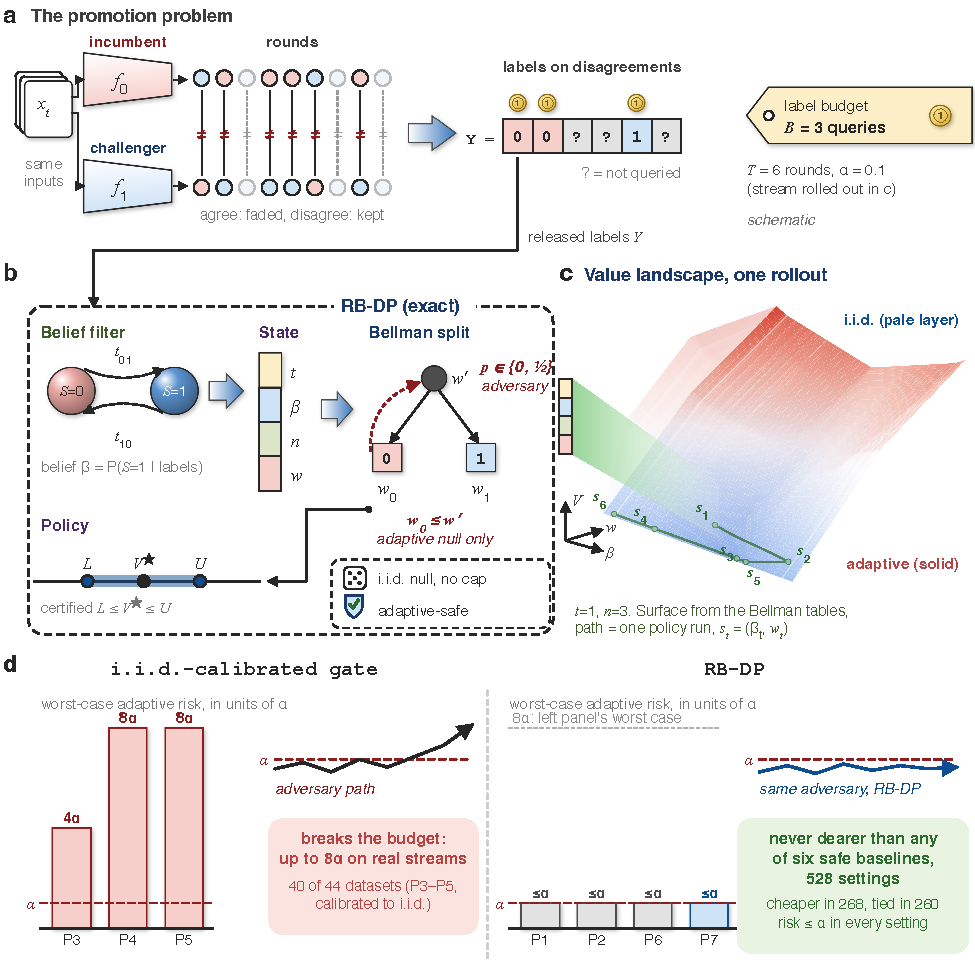
\includegraphics[width=\linewidth]{figures/fig_overview.pdf}
\caption{How RB-DP works (schematic, except where noted). (a) An incumbent and a challenger score the same inputs. Rounds where they agree are dropped. On the disagreements, up to $B$ labels can be bought, which gives a stream such as $Y=0\,0\,?\,?\,1\,?$, where ? means not queried. (b) RB-DP filters a two-state hidden regime with switching probabilities $t_{01}$ and $t_{10}$ and carries the state $(t,\beta,n,w)$, where $w$ is the risk budget. After a query the adversary picks $p\in\{0,1/2\}$ and the budget $w'$ splits into $w_0$ and $w_1$ for the two label branches. The adaptive null adds the cap $w_0\le w'$ (Theorem~\ref{thm:reduction}). The extracted policy gives the sandwich $L\le V^\star\le U$ (Corollary~\ref{cor:sandwich}). (c) Computed: the value of information at $t=1$ with $n=3$ labels left over a grid of beliefs $\beta$ and budgets $w$, from the lattice solver (same cell as Figure~\ref{fig:lattice}). The solid surface is the adaptive null and the pale layer above it the i.i.d.\ null; the gap is the premium. The green path is one simulated run of the extracted policy, with $s_t=(\beta_t,w_t)$ drawn on the surface at $t=1$, $n=3$; the strip in (a) is that run. (d) Computed from the baseline panel (Section~\ref{sec:real}): the i.i.d.-calibrated rules P3, P4 and P5 reach $4\alpha$, $8\alpha$ and $8\alpha$ in the worst case, while P1, P2, P6 and RB-DP (P7) stay within $\alpha$, and RB-DP is never dearer than the six causal-safe baselines in 468 settings. The adversary paths in (d) are drawn for illustration.}
\label{fig:overview}
\end{figure}

\subsection{The worst-case risk-to-go}

A behavioural strategy $\sigma$ gives, at each pre-promotion history $h$, a probability $\pi(h)$ of promoting now and, given no promotion, a probability $\kappa(h)$ of querying. Let $R_\sigma(h)=\sup_{\nu\in\mathcal{N}_X}\PP_{\nu,\sigma}(\text{promotion at some time}\ge t\mid h)$ be its worst-case risk-to-go, and let $h\cdot\varnothing$ and $h\cdot y$ be the successors after no query and after a query with label $y$.

\begin{lemma}[Risk recursion]
\label{lem:risk}
With $m(a,b)=\max\{a,(a+b)/2\}$ for the adaptive class and $m(a,b)=(a+b)/2$ for the i.i.d.\ null, and $R_\sigma\equiv 0$ after $T$,
\[
R_\sigma(h)=\pi(h)+(1-\pi(h))\Big[(1-\kappa(h))R_\sigma(h\cdot\varnothing)+\kappa(h)\,m\big(R_\sigma(h\cdot 0),R_\sigma(h\cdot 1)\big)\Big].
\]
\end{lemma}

The adaptive class is a product over histories, so the null's choice at $h$ and its choices in the two subtrees are free of one another. The risk-to-go after a query is $(1-p)R_\sigma(h\cdot 0)+pR_\sigma(h\cdot 1)$, linear in $p\in[0,1/2]$, so the supremum is attained at $p=0$ or $p=1/2$, which gives $m$. Two conditions are needed (Appendix~\ref{app:proofs}): the learner draws its coins fresh at each step and the null does not see them, and at $d=1$ the null knows no label the learner has not seen. If the null could see a pre-drawn plan, the recursion would fail: with $T=2$ and promotion probability $1/2$ after either label, behavioural risk is $1/2$ while a null that sees the plan reaches $5/8$.

\subsection{Exact reduction}

Lemma~\ref{lem:risk} says that the only thing the future needs to know about the past, as far as risk is concerned, is a single number: how much worst-case promotion probability the continuation may still use. This suggests carrying it as a state.

\begin{definition}[Risk-budget value]
$W_X(t,\beta,n,w)$ is the infimum of expected alternative cost from time $t$ on, over continuation strategies started unpromoted at belief $\beta$ with $n$ labels left whose worst-case risk-to-go is at most $w$.
\end{definition}

Let $\beta'$ be the one-step propagated belief, $\beta_y$ the posterior after label $y$ propagated one step, $\PP(y\mid\beta)$ the predictive label probability, and $P(t,n,\beta)$ the optimal cost of promoting at $t$ and playing the unconstrained belief DP afterwards.

\begin{theorem}[Exact reduction, $d=1$]
\label{thm:reduction}
$V^\star_X=W_X(1,\beta_1,B,\alpha)$. Moreover $W_X(T+1,\cdot)=0$ and, for $t\le T$, $W_X(t,\beta,n,\cdot)$ is the lower convex hull on $[0,1]$ of $f(w')=\min\{C_N(w'),C_Q(w')\}$ for $w'<1$ and $f(1)=\min\{C_N(1),C_Q(1),P(t,n,\beta)\}$, where
\begin{align*}
C_N(w')&=\pos(\beta)+W_X(t+1,\beta',n,w'),\\
C_Q(w')&=\pos(\beta)+c+\min\Big\{\textstyle\sum_{y}\PP(y\mid\beta)\,W_X(t+1,\beta_y,n-1,w_y)\;:\;m(w_0,w_1)\le w',\ w_y\in[0,1]\Big\},
\end{align*}
and $C_Q\equiv+\infty$ if $n=0$. $W_X$ is nonincreasing and convex in $w$ and concave in $\beta$.
\end{theorem}

The hull is essential. The learner may randomise between promoting, continuing without a query and querying, and between continuation budgets; this is exactly a mixture of points on the graph of $f$ with mean abscissa at most $w$. A first version of the programme without the hull exceeded the certified exact optimum on a $T=5$, $B=2$ cell (2.4461 against 2.44189), which is how we found it.

\begin{corollary}[The premium is one constraint]
\label{cor:oneconstraint}
The adaptive and i.i.d.\ programmes differ only in $m$: the adaptive programme adds $w_0\le w'$ to the i.i.d.\ constraint $(w_0+w_1)/2\le w'$. The premium $\Gamma$ is the cost of forbidding the risk budget to grow after a label that favours the incumbent.
\end{corollary}

The interpretation is direct (Figure~\ref{fig:split}). Under the i.i.d.\ null a learner can ``borrow'' risk: after a label $Y=0$ it may plan to promote with higher probability than its current budget, provided it plans lower after $Y=1$, because the two branches are averaged. Under the adaptive null the branch $Y=0$ can be forced (by $p=0$), so its budget may not exceed the current one.

\begin{figure}[t]
\centering
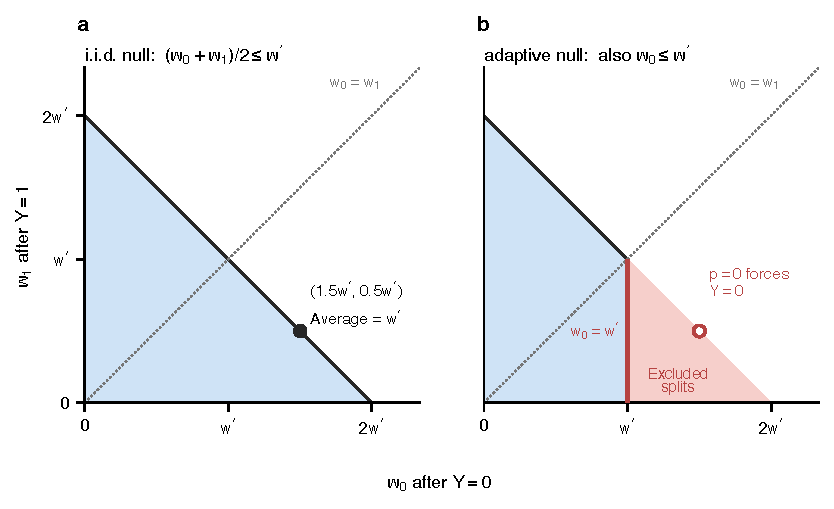
\includegraphics[width=\linewidth]{figures/fig_split.pdf}
\caption{Feasible child risk budgets $(w_0,w_1)$ after a query, for a parent budget $w'$. (a) Under the i.i.d.\ null the two branches are averaged, so the learner may give the branch after $Y=0$ more than $w'$ if it gives the other branch less. (b) The adaptive null can make $Y=0$ certain, so it adds the cap $w_0\le w'$ (Corollary~\ref{cor:oneconstraint}). The red triangle is the region the adaptive programme loses; every unit of premium $\Gamma$ comes from optimal i.i.d.\ plans that use it. Conceptual figure, no data.}
\label{fig:split}
\end{figure}

\subsection{The dyadic lattice}

The $w$ coordinate is continuous. The next result shows that it can be discretised without loss.

\begin{theorem}[Dyadic lattice]
\label{thm:lattice}
Let $D_n=\{k/2^n:k=0,\dots,2^n\}$. For $X\in\{\mathrm{causal},\mathrm{IID}\}$ and every $t,\beta,n$, $W_X(t,\beta,n,\cdot)$ is piecewise linear with all breakpoints in $D_n$.
\end{theorem}

The proof (Appendix~\ref{app:lattice}) is a backward induction with three steps. The no-query branch inherits breakpoints from the next layer. In the i.i.d.\ query branch the constraint is tight and $C_Q(w')$ is an infimal convolution of two convex piecewise-linear functions evaluated at $2w'$; its breakpoints are partial sums of piece lengths, all multiples of $2^{-(n-1)}$, so after halving they lie in $D_n$: one query adds one bit. In the adaptive branch the extra cap $w_0\le w'$ binds on a set whose boundary is where the minimising staircase crosses the diagonal $w_0=w_1$, which happens only at points of $D_{n-1}$. Finally, a lower convex hull introduces no new breakpoints.

\begin{figure}[t]
\centering
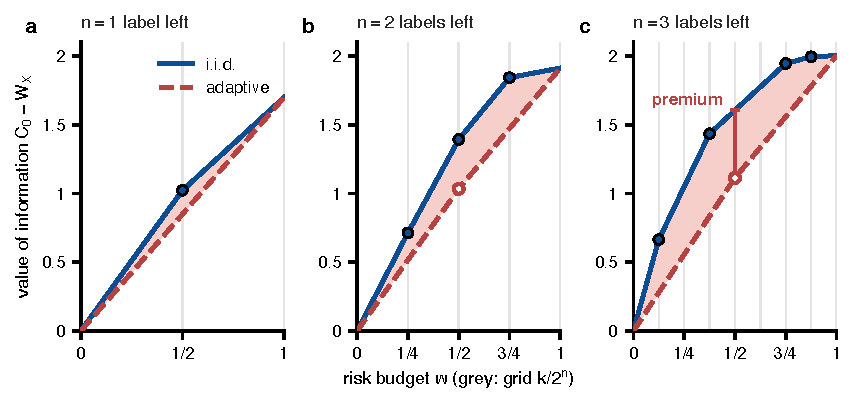
\includegraphics[width=\linewidth]{figures/fig_lattice.pdf}
\caption{The value is piecewise linear in $w$ with breakpoints on the dyadic grid. Each curve is the value of information $C_0-W_X(1,\beta_1,n,w)$ from the lattice solver on one cell ($T=6$, $B=3$, both transition probabilities $19/20$, $e_1=1-e_0=49/50$, $\alpha=1/10$, $G=401$), for $n=1,2,3$ labels remaining under the i.i.d.\ null (blue, filled markers) and the adaptive null (red dashed, open markers). Markers are the kinks of each curve. Every kink lies on $\{k/2^n\}$ (grey lines), and the script asserts this. The gap between the curves is the cost of the extra cap $w_0\le w'$. Computed by \texttt{risk\_budget\_dp\_fast.py}.}
\label{fig:lattice}
\end{figure}

\begin{corollary}[Exact finite programme]
\label{cor:finite}
Let $N$ be a multiple of $2^B$ and restrict every risk budget to $\{j/N\}$. The restricted programme has the same value as $W_X$ at every grid point; at an off-grid $\alpha$, $W_X(\cdot,\alpha)$ is the linear interpolation of its two grid neighbours.
\end{corollary}

The condition that $2^B$ divides $N$ matters. A grid of $3d_\alpha$ points that contains $\alpha$ but is not a multiple of $2^B$ was worse than exact in 9 of 40 stress runs, by up to $6.6\times10^{-3}$ (Appendix~\ref{app:stress}).

\subsection{Algorithm and certified bounds}

Algorithm~\ref{alg:rbdp} summarises the solver. We use a grid of $G$ beliefs that contains 0 and 1, with linear interpolation between grid points, and the $w$ lattice of Corollary~\ref{cor:finite} with $N=10\cdot 2^B$ (so that $\alpha=1/10$ is a grid point).

\begin{algorithm}[t]
\caption{RB-DP (delay 1)}
\label{alg:rbdp}
\begin{algorithmic}[1]
\REQUIRE horizon $T$, budget $B$, costs $c,k$, level $\alpha$, chain $(t_{01},t_{10},e_0,e_1)$, prior, mode $X$
\STATE belief grid $\{\beta_g\}_{g=1}^G\ni 0,1$; risk lattice $\{j/N\}$ with $2^B\mid N$
\STATE $W(T+1,\cdot,\cdot,\cdot)\leftarrow 0$; precompute post-promotion values $P(t,n,\beta_g)$ by the belief DP
\FOR{$t=T,\dots,1$}
  \FOR{each $n\le B$ and each $\beta_g$}
    \STATE $C_N(w')\leftarrow\pos(\beta_g)+W(t+1,\beta_g',n,w')$ (interpolated in $\beta$)
    \STATE $C_Q(w')\leftarrow\pos(\beta_g)+c+\min_{m_X(w_0,w_1)\le w'}\sum_y\PP(y\mid\beta_g)W(t+1,\beta_{g,y},n-1,w_y)$ \COMMENT{slope merge; extra cap $w_0\le w'$ if $X$ = causal}
    \STATE $f\leftarrow\min(C_N,C_Q)$; $f(1)\leftarrow\min(f(1),P(t,n,\beta_g))$
    \STATE $W(t,\beta_g,n,\cdot)\leftarrow$ lower convex hull of $f$ on the lattice; record the hull vertices as the policy
  \ENDFOR
\ENDFOR
\STATE $L\leftarrow W(1,\beta_1,B,\alpha)$
\STATE extract the policy; evaluate its cost $U$ exactly on its forward tree and its worst-case risk by Lemma~\ref{lem:risk}
\RETURN $L$, $U$, policy
\end{algorithmic}
\end{algorithm}

\begin{corollary}[Certified sandwich and cost]
\label{cor:sandwich}
The programme has $T(B+1)G(N+1)$ states, and each backward step costs $O(N\log N)$ per belief row. Since $W$ is concave in $\beta$ and the Bellman operator is monotone, belief interpolation gives $L\le V^\star_X$. The extracted policy, run on exact beliefs, is a valid strategy; if its exactly evaluated risk is at most $\alpha$, its exactly evaluated cost $U$ satisfies $V^\star_X\le U$. Thus $L\le V^\star_X\le U$, and the only slack comes from belief interpolation.
\end{corollary}

In the symmetric chains below the belief stays at $1/2$ until the first label, and $L=U$ to twelve digits in the parameter region of the theorems in Section~\ref{sec:premium}.

%=====================================================================
\section{What the premium looks like}
\label{sec:premium}

Corollary~\ref{cor:oneconstraint} turns the premium into a question about one constraint. When does it bind?

\paragraph{Persistent regimes: no premium at one label.} If the chain is persistent ($t_{01}+t_{10}\le 1$) and the alternative's marginal probability of a challenger win at the query time is at least $1/2$, then with a single label ($B=1$) some optimal plan promotes on a monotone event of the label tape, for every Lagrange multiplier. A monotone promotion event has the same risk under every adaptive null as under fair coins, by a coupling of the null tape with an i.i.d.\ tape, so $\Gamma=0$ (Proposition~\ref{prop:z1} below; proof in Appendix~\ref{app:structure}). With $B\ge 2$ this fails: there are persistent cells with a small positive premium (e.g.\ $\Gamma=1.3\times10^{-4}$ at $T=4$, $B=2$, $d=2$). In the synthetic grid of Section~\ref{sec:synthetic} and on the persistent real streams, the premium is zero or small; the large premia come from anti-persistent regimes.

\begin{proposition}[No premium at one label in persistent regimes]
\label{prop:z1}
Let $B=1$ and let $T$, $d\ge1$, $c,k\ge0$ and $\alpha\in[0,1]$ be arbitrary. If $t_{01}+t_{10}\le1$, $e_1>e_0$, and $\PP_A(Y_\tau=1)\ge1/2$ for every query time $\tau\le T-d$, then $\Gamma=0$.
\end{proposition}

\paragraph{Anti-persistent regimes: a premium that does not vanish.} Take the symmetric stationary anti-persistent chain $t_{01}=t_{10}=t\in(1/2,1)$, with $r=2t-1$, emissions $(e,1-e)$ and $g=(1-2e)^2$. Here a label that favours the incumbent predicts that the challenger will be better shortly afterwards, so the best i.i.d.\ plan promotes after $Y=0$ with high probability. That is the branch an adaptive null can force. The following results are proved in Appendix~\ref{app:structure}.

\begin{theorem}[Premium bounds; $d=1$ unless stated]
\label{thm:premium}
\begin{enumerate}
\item ($B=1$, $d$ odd, $\alpha\le1/2$, $c=k=0$.) $\rhoG$ does not depend on $\alpha$, and $\inf_{T\ge d+1}\rhoG(T)=\lim_T\rhoG(T)=(1-r)/2$.
\item ($B=2$, $k=0$, $d$ odd, $c=0$, $\alpha\le 1/2$.) $\liminf_T\rhoG(T)\ge(1-r)/(2(3+r))$.
\item ($B\le 6$, $c=k=0$, $\alpha=1/10$, $r\in(1/200,1/100)$, $g\in(2/5,1/2)$.) $\rhoG(T)\ge 0.10$ for every $T\ge 20$; the bounds for $B=3,4,5,6$ are $19/101$, $13/84$, $40/303$ and $13/118$.
\item (Any fixed $B\ge 1$, $c=k=0$, $\alpha=1/10$, $2/5<g<1/2$, $0<r<1/[16(B+2)(6B^3+3B+2)]$.) $\rhoG(T)\ge 3/[8(B+2)]$ for every $T\ge 3B$.
\end{enumerate}
\end{theorem}

Part 4 holds for each fixed budget on a region that shrinks as $B^{-4}$, with a bound that decays as $B^{-1}$; we do not have a single region and constant uniform over unbounded $B$. The theorems cover small parameter regions. RB-DP is what lets us see the whole curve (Section~\ref{sec:e3}): the measured limits sit at or above every proved bound, and for $B=2$ the measured limit is $(1-r)/(3+r)$, exactly twice the bound in part 2 (a numerical observation).

%=====================================================================
\section{Synthetic experiments}
\label{sec:synthetic}

All cells in this section use $d=1$. Solver: lattice mode, $N=10\cdot2^B$, $G=401$ unless stated, float64. Every result file records the script and solver hashes, grid, seed and per-cell run time.

\subsection{Agreement with certified optima}
\label{sec:e1}

We compared RB-DP with an exact sequence-form solver that returns rational intervals of width about $10^{-12}$.
\begin{itemize}
\item \textbf{150 certified cells} from an earlier scaling study ($B\le4$, $T\le16$, $t\in\{2/3,3/4,9/10\}$, $k\in\{0,1/50\}$, $\alpha\in\{1/20,1/10,1/4\}$), all with certified $\Gamma>0$. With the first, uniform-grid version of the solver, 148 agree to $1.1\times10^{-14}$. Two $B=4$ cells were off by at most $2.5\times10^{-3}$ because that grid was not dyadic; in lattice mode they are exact (3.145989478 and 5.448796194).
\item \textbf{40 fresh random cells} (seed 20261113; $T\le8$, $B\le3$, asymmetric chains, $c\in\{0,1/100\}$, $k\le1/10$): the exact value lies in $[L,U]$ for all 40 in both modes, and $U$ equals it to round-off in 38.
\item \textbf{60 certified premium cells} in lattice mode: maximum $|\rhoG|$ deviation $4.2\times10^{-13}$.
\end{itemize}
No bound was violated in any of the 190 cells. An independent check by a separate solver reproduced the exact optimum with its own linear programme on 10 cells to $1.3\times10^{-15}$, and verified Theorem~\ref{thm:lattice} in exact rational arithmetic on 45{,}768 value rows with no breakpoint off the dyadic grid.

\subsection{Scaling}
\label{sec:e2}

% Source: docs/paper4_continuation/rbdp/E2_E3_SCALING_PREMIUM.md section 4 (shared machine; timings pessimistic).
\begin{table}[t]
\centering
\caption{Run time of RB-DP (one CPU thread, shared machine; $t=3/4$, $e=1/10$, adaptive mode, $G=401$). $N_w$ is the size of the risk lattice. Left: growth in $T$ at $B=3$. Right: growth in $B$ at $T=32$.}
\label{tab:scaling}
\small
\begin{tabular}{rrr@{\qquad}rrr}
\toprule
$T$ & $B$ & seconds & $T$ & $B$ ($N_w$) & seconds\\
\midrule
16 & 3 & 0.6 & 32 & 1 (21) & 0.2\\
32 & 3 & 1.2 & 32 & 2 (41) & 0.4\\
64 & 3 & 2.2 & 32 & 4 (161) & 2.6\\
128 & 3 & 4.4 & 32 & 6 (641) & 15.5\\
256 & 3 & 8.3 & 32 & 8 (2561) & 122.1\\
\bottomrule
\end{tabular}
\end{table}

Table~\ref{tab:scaling} shows time linear in $T$ and exponential in $B$, as Corollary~\ref{cor:sandwich} predicts; a rough rule is $1.6\times10^{-3}\,T\,B\,2^B$ seconds per mode. For comparison, the exact sequence-form solver took 37 to 71\,s at $T=10$ and timed out at 3{,}600\,s on the cell $T=16$, $B=3$, $t=63/125$, $e=3/20$. RB-DP solves that cell in 0.4\,s with $L=U$ to twelve digits.

\subsection{The premium at long horizons}
\label{sec:e3}

% Source: docs/paper4_continuation/rbdp/RESULTS.md and E2_E3_SCALING_PREMIUM.md section 1.
\begin{table}[t]
\centering
\caption{Relative premium $\rhoG$ at the largest horizon run ($T=100$; $T=200$ for $t=3/4$, $B\le5$), $\alpha=1/10$, $e=1/10$, $c=k=0$, $d=1$, symmetric stationary chains. $L$--$U$ brackets are at most $7\times10^{-4}$ wide in $\rhoG$. For $t=3/4$ we also ran $B=7$ (0.3680 at $T=100$) and $B=8$ (0.4018 at $T=64$, not yet level).}
\label{tab:e3}
\small
\begin{tabular}{lcccccc}
\toprule
$t$ & $B=1$ & $B=2$ & $B=3$ & $B=4$ & $B=5$ & $B=6$\\
\midrule
2/3 & 0.3333 & 0.2000 & 0.1429 & 0.1111 & 0.1135 & 0.1404\\
3/4 & 0.2500 & 0.1429 & 0.1000 & 0.1379 & 0.2139 & 0.3034\\
9/10 & 0.1000 & 0.0526 & 0.1460 & 0.2218 & 0.2688 & 0.2762\\
\bottomrule
\end{tabular}
\end{table}

For every $B\le6$ and $t\in\{2/3,3/4,9/10\}$, $\rhoG(T)$ decreases over small $T$ and then levels off at a positive value; by $T=48$ to $100$ consecutive values agree to about three decimals (Figure~\ref{fig:premium}, Table~\ref{tab:e3}; the values are in Appendix~\ref{app:curves}).

\begin{figure}[t]
\centering
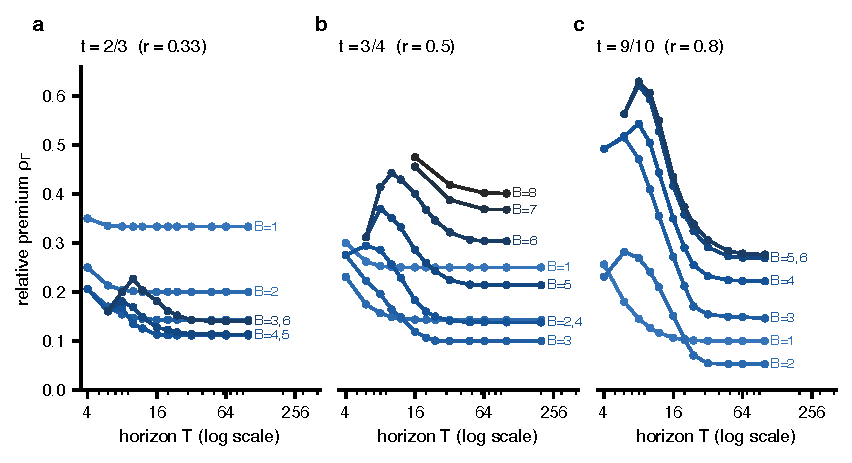
\includegraphics[width=\linewidth]{figures/fig_premium.pdf}
\caption{Relative premium $\rhoG$ against horizon $T$ for label budgets $B=1,\dots,6$ (and $B=7,8$ for $t=3/4$), symmetric anti-persistent chains with switching probability $t$ ($r=2t-1$), $e=1/10$, $\alpha=1/10$, $c=k=0$, $d=1$. Darker lines are larger budgets; labels such as ``B=3,6'' mark curves that end within 0.01 of each other. Every curve levels off above zero; the $B=8$ curve has not fully levelled at $T=64$. Source: \texttt{rbdp/results/e2e3\_fast\_cells.jsonl}, 223 cells.}
\label{fig:premium}
\end{figure} No curve heads to zero. The premium is not monotone in $B$: it falls for small budgets and rises again for larger ones. In every cell of the table the i.i.d.-mode policy, evaluated against the adaptive null, has worst-case risk 0.2 to 0.4 against a budget of 0.1, while the adaptive-mode policy sits at 0.1000.

\paragraph{Agreement with the theory.} The $B=1$ values match the closed form of Theorem~\ref{thm:premium}(1) to $2.3\times10^{-12}$ at every $T\le200$. In the parameter region of parts 3 and 4 ($t=63/125$, $e=3/20$, $g=0.49$), $\rhoG$ at $T\in\{16,20,32\}$ is 0.2470, 0.1975, 0.1645 and 0.1409 for $B=3,\dots,6$, above the proved bounds 0.1881, 0.1548, 0.1320 and 0.1102.

\subsection{Comparison with safe baselines}
\label{sec:e4}

We compare RB-DP with three causal-safe alternatives and one unsafe one, all calibrated to $\alpha=1/10$:
(a)~\textbf{i.i.d.-optimal + repair}: the i.i.d.-optimal policy mixed at the root with never-promote until its worst-case adaptive risk is $\alpha$;
(b)~\textbf{e-process gate}: a stake-1 betting wealth $\prod(1+(2Y_i-1))$ on queried labels, with promotion when it reaches a threshold $\theta\in\{2,4,8\}$, $\theta\le 2^B$, mixed with never-promote at rate $\min(1,\alpha\theta)$; it is safe by Ville's inequality \citep{ville1939etude,ramdas2023gametheoretic}, and we report the best $\theta$;
(c)~\textbf{never promote};
(d)~\textbf{i.i.d.-optimal} without repair, whose adaptive risk we report.

% Source: docs/paper4_continuation/rbdp/E1_E4_VALIDATION_BASELINES.md, E4 table (selected rows; full table in appendix).
\begin{table}[t]
\centering
\caption{Share of RB-DP's value of information captured by safe baselines, and worst-case adaptive risk of the unrepaired i.i.d.-optimal policy ($\alpha=1/10$, $e=1/10$, $d=1$). ``anti $t$'': symmetric anti-persistent chain; ``pers $t$'': persistent; ``asym'': $(t_{01},t_{10})=(9/10,2/3)$. Full table: Appendix~\ref{app:e4}.}
\label{tab:e4}
\small
\begin{tabular}{rlrcrrrr}
\toprule
$T$ & chain & $B$ & $c,k$ & VOI RB-DP & repair & e-gate & i.i.d.-opt risk$/\alpha$\\
\midrule
8 & anti 2/3 & 3 & 0, 0 & 0.0439 & 0.591 & 0.818 & 2.00\\
8 & anti 9/10 & 3 & 0, 0 & 0.1637 & 0.473 & 0.852 & 4.00\\
8 & anti 3/4 & 3 & 1/100, 1/20 & 0.0457 & 0.888 & 0.803 & 1.33\\
32 & anti 3/4 & 3 & 0, 0 & 0.0959 & 0.556 & 0.889 & 2.00\\
32 & anti 9/10 & 3 & 0, 0 & 0.3676 & 0.591 & 0.957 & 2.00\\
32 & asym & 3 & 0, 0 & 0.6552 & 0.602 & 1.000 & 2.00\\
32 & pers 1/10 & 3 & 0, 0 & 0.7545 & 1.000 & 1.000 & 1.00\\
32 & pers 1/4 & 3 & 1/100, 1/20 & 0.1210 & 1.000 & 1.000 & 1.00\\
\bottomrule
\end{tabular}
\end{table}

Across 40 cells (Appendix~\ref{app:e4}), no safe baseline exceeds RB-DP. On anti-persistent chains without costs the repair captures 0.47 to 0.68 of RB-DP's value of information and the e-process gate 0.74 to 0.96. With $c=1/100$, $k=1/20$ the order flips: 0.89 to 0.92 for the repair and 0.72 to 0.80 for the gate. The e-gate equals RB-DP on the two $T=32$ asymmetric cells. On persistent chains the i.i.d.\ optimum is already causal-safe and all methods tie. The unrepaired i.i.d.\ policy has more value of information than RB-DP, but it is not admissible: its adaptive risk is $2\alpha$ in every anti-persistent cell without costs, $4\alpha$ in one, and $1.33\alpha$ with costs.

%=====================================================================
\section{Real streams}
\label{sec:real}

The real-data study asks two questions. Under models fitted to real binary streams, is the premium positive and does i.i.d.\ calibration break the adaptive budget? And when the policies are run on real held-out label sequences, how do their realised costs compare? Every phase followed a written protocol fixed before the phase was run; no repository holdout was opened.

\paragraph{Streams and fitting.} We fit the two-state model of Section~\ref{sec:setup} by maximum likelihood to each stream and evaluate it with the solver at $d=1$, $T\in\{16,32\}$, $B\in\{1,\dots,4\}$, $\alpha=0.1$, in both label orientations. A dataset counts as supporting when some cell has $\rhoG>10^{-3}$, value of information $C_0-\Vi\ge0.1$, and at most one of five time-shuffles of the stream is also positive. The shuffle control removes temporal structure while keeping the marginal rate. Streams built by differencing a series (``did it rise?'') were excluded after a white-noise control showed that they pass the screen at the same rate as i.i.d.\ Gaussian noise (Appendix~\ref{app:realdetails}).

\begin{figure}[!tbp]
\centering
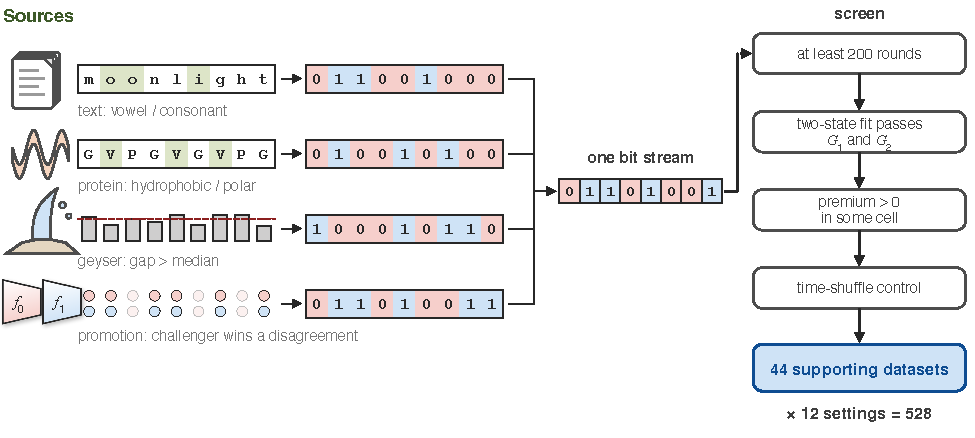
\includegraphics[width=\linewidth]{figures/fig_screen.pdf}
\caption{Of the 48 sources screened in Phases 10 and 10b, 4 pass and join 35 from earlier phases, giving 39 supporting datasets. (a) Each source becomes one binary stream built from levels only: differenced series are dropped, because white noise passes the screen as often as real streams (2 of 24 against 13 of 150). The icons and snippets are illustrative, but the bit rules are the pipeline's (vowels, hydrophobic residues, gaps above the median). Streams then pass a length and availability check (at least 200 rounds; 35 remain), the two-state fit gates $G_1$ and $G_2$ (17), a premium in some cell (4) and a time-shuffle control (4). $G_1$ requires the fit to beat an i.i.d.\ model on held-out data and $G_2$ requires a valid chain ($e_0<1/2<e_1$, transitions in $[0.01,0.99]$). The 39 datasets give 468 panel settings. (b) Outcome of the 48 sources. (c) The 39 supporting datasets by type. Sources: \texttt{LEDGER\_PHASE10.md}, \texttt{REAL\_CHAINS.md}, \texttt{attempts*.jsonl}, \texttt{phase9\_replay.jsonl}.}
\label{fig:screen}
\end{figure}

\subsection{Thirty-nine datasets with a positive premium}

% Source: docs/paper4_continuation/rbdp/real_data/REAL_CHAINS.md (Phases 4b-7).
The study found 39 supporting datasets (Table~\ref{tab:real35} in Appendix~\ref{app:realdetails}): 18 texts in 18 languages read as vowel/consonant streams, five protein sequences read as hydrophobic/polar streams (four elastins and a spider-silk spidroin), the Old Faithful geyser in three recordings \citep{azzalini1990faithful} and the Grand geyser, and twelve model-promotion streams. In a promotion stream $Y_t=1$ when the challenger is right and the incumbent wrong on a disagreement round, computed from cached paired losses of chronologically trained incumbent and challenger models on standard drift benchmarks (air quality, energy, electricity meters and prices, exchange rates, activity recognition, forest cover). This is the paper's own setting. All 39 pass the shuffle control with zero of five shuffles positive. The best-cell $\rhoG$ ranges from 0.001 (Tetouan power) to 0.44 (geyser), and in the best cell the i.i.d.-optimal policy's adaptive risk is 0.15 to 0.8 against $\alpha=0.1$. Most supporting streams are anti-persistent ($r_1$ from $-0.56$ to $-0.13$); the spidroin and eleven of the twelve promotion streams are persistent with noisy emissions and still have a positive premium at $T=32$, $B=4$. Under the same rule we screened 48 further benchmark and alternation sources (drift benchmarks, further OpenML tables, further geysers), and 4 qualified; the covtype, Elec2 and two geyser rows above are those 4. The other 44 were null, too short, rejected by the two-state fit, or unavailable. Streams with $r_1$ near zero show no premium, as Section~\ref{sec:premium} predicts. The screening record for all 48 is in the supplementary material (\texttt{LEDGER\_PHASE10.md}).

\paragraph{Baseline panel.} On each of the 39 fitted chains we ran seven policies over 12 settings ($T\in\{16,32\}$, $B\in\{2,3,4\}$, $\alpha\in\{0.05,0.1\}$; 468 settings), with exact cost and exact worst-case adaptive risk: P1 fixed-sample test, P2 count SPRT \citep{wald1945sequential}, P3 HMM-filter threshold, P4 myopic value-of-information rule, P5 i.i.d.-optimal planner, P6 e-process gate, and P7 RB-DP. P3 to P5 are calibrated to the i.i.d.\ null as a practitioner would. We then added causal-safe versions of the three i.i.d.-calibrated rules: P3c and P4c recalibrated to exact adaptive risk $\alpha$, and P5r, the cheaper of a deflated-level re-solve and mixing with never-promote.

% Source: REAL_CHAINS.md, Phase 7 T16/32 panel and Phase 9 panel.
\begin{itemize}
\item \textbf{Safety.} RB-DP, P1, P2, P6 and the repaired P3c, P4c, P5r are causal-safe in all 468 settings. The i.i.d.-calibrated P3, P4, P5 break the adaptive budget on 35 of 39 datasets, with worst cases $4\alpha$, $8\alpha$ and $8\alpha$ (geysers); they violate it in 324, 304 and 288 settings.
\item \textbf{Cost.} Against the best of the six safe baselines per setting, RB-DP is cheaper in 212, ties in 256 and is more expensive in 0. The median share of RB-DP's value of information captured by the recalibrated rules is 0.29 (P3c), 0.35 (P4c) and 0.60 (P5r).
\end{itemize}
Since RB-DP is optimal in the fitted model, it cannot lose in-model; the panel measures by how much the alternatives fall short. Figure~\ref{fig:real}(a) shows the worst adaptive risk per dataset for each policy.

\begin{figure}[t]
\centering
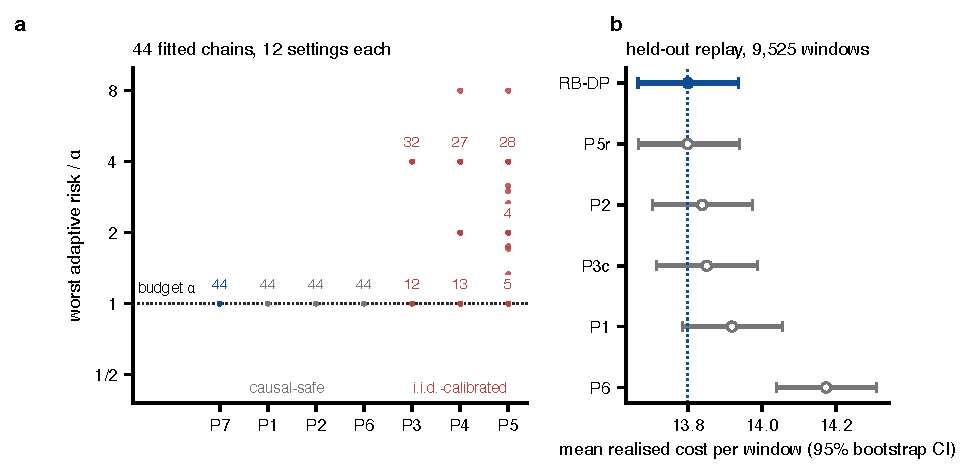
\includegraphics[width=\linewidth]{figures/fig_real.pdf}
\caption{Real streams. (a) For each of the 39 fitted chains, the largest worst-case adaptive risk over the 12 panel settings, in units of $\alpha$ (log scale, points jittered). RB-DP (P7, blue) and the safe baselines P1, P2, P6 sit at $\alpha$; the i.i.d.-calibrated rules P3, P4, P5 exceed it on 35 of 39 datasets, by up to $8\alpha$. (b) Held-out replay: pooled mean realised cost per window of the safe policies with 95\% window-bootstrap intervals (2{,}000 resamples, seed 20261119). P4c (15.83) is off the scale and omitted. Sources: \texttt{phase7\_baselines\_T16\_32/settings.jsonl}, \texttt{phase10\_baselines/settings.jsonl}, \texttt{phase9\_replay.jsonl}.}
\label{fig:real}
\end{figure}

\subsection{Census and held-out replay on promotion streams}

The 39 datasets were selected by the premium screen. To see what happens on promotion streams in general, we ran two further analyses over the whole inventory of 114 cached promotion datasets, fitting each model on the first half of each dataset's episodes only.

\paragraph{Census.} Of the 102 datasets with enough fit-set rounds, the value of information is large (median 1.29, 90th percentile 8.5), the premium is mostly zero (median $\rhoG=0$; 11 of 102 above $10^{-3}$, mostly exchange-rate pairs), and the i.i.d.-optimal policy's adaptive risk is at $\alpha$ for most datasets (75th percentile 0.10, 90th percentile 0.145, maximum 0.40). Promotion streams are mostly persistent (median $r_1=+0.30$): the challenger's advantage comes in runs, and Section~\ref{sec:premium} predicts little premium for such regimes.

\paragraph{Replay.} On the 100 datasets with enough held-out rounds we cut every held-out episode into non-overlapping windows of $T=32$ disagreement rounds (9{,}525 windows) and ran every policy, calibrated on the fit half, on the real label sequence of each window ($B=4$, $\alpha=0.1$, $c=0.01$, $k=0$). Realised cost replaces predicted probabilities in the cost model by the real labels. Step-by-step executors of all policies matched their exact in-model costs on three datasets over 20{,}000 simulated windows each ($|z|\le2.16$).

% Source: REAL_CHAINS.md Phase 8 replay table and Phase 9 replay table.
\begin{table}[t]
\centering
\caption{Held-out replay on 9{,}525 real windows from 100 promotion datasets ($T=32$, $B=4$, $\alpha=0.1$, $c=0.01$). Mean realised cost with 95\% window-bootstrap interval, paired difference to RB-DP (negative: RB-DP cheaper), and number of datasets on which the policy's exact adaptive risk under the fitted model exceeds $\alpha$.}
\label{tab:replay}
\small
\begin{tabular}{lccc}
\toprule
policy & mean realised cost & RB-DP $-$ policy & datasets with risk $>\alpha$\\
\midrule
never promote & 17.964 [17.808, 18.123] & & 0\\
P1 fixed-sample & 13.918 [13.784, 14.050] & $-0.119$ [$-0.176$, $-0.063$] & 0\\
P2 count SPRT & 13.838 [13.701, 13.971] & $-0.039$ [$-0.097$, 0.019] & 0\\
P6 e-process gate & 14.173 [14.039, 14.310] & $-0.374$ [$-0.443$, $-0.301$] & 0\\
P3c filter, recalibrated & 13.850 [13.713, 13.987] & $-0.051$ [$-0.108$, 0.006] & 0\\
P4c myopic VOI, recalibrated & 15.834 & $-2.035$ [$-2.190$, $-1.890$] & 0\\
P5r i.i.d.-optimal, repaired & 13.799 [13.665, 13.938] & $+0.0005$ [$-0.009$, 0.009] & 0\\
\textbf{P7 RB-DP} & \textbf{13.799} [13.664, 13.936] & & \textbf{0}\\
\midrule
P3 filter (i.i.d.-calibrated) & 13.849 [13.713, 13.982] & & 21\\
P4 myopic VOI (i.i.d.-calibrated) & 15.763 [15.615, 15.915] & & 12\\
P5 i.i.d.-optimal & 13.803 [13.672, 13.939] & & 5\\
\bottomrule
\end{tabular}
\end{table}

Table~\ref{tab:replay} shows that RB-DP has the lowest pooled realised cost among the safe policies. It is significantly cheaper than P1, P6 and P4c, not distinguishable from P2 and P3c, and tied with the repaired i.i.d.\ planner P5r (difference $0.0005$, interval $[-0.009,0.009]$). The i.i.d.-calibrated policies that come close in cost do so while breaking the adaptive budget on 21 (P3) and 5 (P5) datasets. Per dataset, against the cheapest of the six safe baselines chosen after the fact, RB-DP is below on 1, tied on 40 and above on 59. The tie with P5r is consistent with the census: on persistent promotion streams the adaptive constraint rarely binds, and a repaired i.i.d.\ planner loses little. RB-DP's advantage is the guarantee by construction and the gains on the regimes where the constraint binds.

%=====================================================================
\section{Delay two}
\label{sec:delay2}

At $d=2$ a label queried at $t-1$ is pending at the decision at $t$: the null has seen it and the learner has not. Lemma~\ref{lem:risk} then fails on learner histories, because the null's information is finer than the learner's. The natural extension carries one risk budget per pending value: a pair $(w^0,w^1)$ when a label is pending and a scalar otherwise, with the hull taken on $[0,1]^2$ (Appendix~\ref{app:delay2}). We built this solver; it matches the certified exact optimum on 166 small cells, but it gives an upper bound only and we have no lattice theorem for it. Its long-horizon study (81 cells, $B\le3$, to $T=100$) finds a smaller premium than at $d=1$ in every cell: zero for $B=1$, zero at $T\ge32$ for $B=2,3$ except $t=9/10$, $B=3$ (level at 0.0399). For $B=4$ (24 cells) the premium levels at 0.0331 for $t=3/4$ and 0.1229 for $t=9/10$, and is zero for $t=2/3$. Values past $T=10$ are not certified. Delay $d\ge3$ is not built.

%=====================================================================
\section{Related work}
\label{sec:related}

\paragraph{Sequential testing against composite and adaptive nulls.} Test supermartingales and e-processes give anytime-valid tests against nulls defined by a conditional mean, which include adaptively chosen conditional laws \citep{ramdas2023gametheoretic,waudbysmith2024betting,howard2021timeuniform}; Ville's inequality bounds their crossing probability \citep{ville1939etude}. Our P6 baseline is such a gate. These methods give a valid test for any betting strategy but do not optimise a downstream cost under a label budget. \citet{fauss2020minimax} study minimax sequential tests against rectangular families of conditional laws, with Lagrangian handling of error constraints and least-favourable laws that adapt to the history; our adaptive null is an instance of their family. They do not consider hidden-state alternatives, query budgets, delayed labels or switching, and do not compare the minimax value with a nominal-null design. Active sequential hypothesis testing \citep{naghshvar2013active} and controlled sensing \citep{nitinawarat2013controlled} choose which observation to take, under a single null law.

\paragraph{Constrained and robust POMDPs.} With an i.i.d.\ null our problem is a chance-constrained POMDP, where optimal policies randomise and LP duality over policy mixtures applies \citep{altman1999constrained,yost2000lp,walraven2018column}. Robust MDPs with rectangular uncertainty admit dynamic programmes over the nominal state \citep{iyengar2005robust,nilim2005robust}; for robust POMDPs, \citet{krale2025evaluating} evaluate fixed policies via a nature MDP. Our constraint is on a family of null laws while the objective is under a separate alternative law, so neither formulation applies directly. One-sided partially observable stochastic games carry a scalarised belief of the uninformed player \citep{horak2023solving}; our risk budget plays a similar role for the null's worst case. The exact solver we compare against is a constraint-generation method in the double-oracle family \citep{bosansky2014exact}.

\paragraph{Structural results.} Monotone and threshold policies for POMDPs under TP2 and MLR conditions \citep{krishnamurthy2016pomdp} underlie our zero-premium result for persistent chains at $B=1$; the event-monotonicity and coupling argument we need is different from monotonicity of a policy in belief.

\paragraph{Model promotion and safe deployment.} Conservative and safe policy improvement \citep{wu2016conservative,thomas2015high} constrain the performance of a new policy against a baseline with high probability, typically from logged data under an i.i.d.\ sampling assumption. Our setting is online, label-scarce and asks for type-I control against an adaptive null.

%=====================================================================
\section{Limitations}
\label{sec:limitations}

\begin{itemize}
\item \textbf{Delay and state space.} The exact reduction and lattice theorem are for $d=1$ and a two-state alternative. The two-state restriction is used only for the one-dimensional belief grid; the proofs do not need it. At $d=2$ we have an upper-bound solver and no lattice theorem.
\item \textbf{Exponential in $B$.} The lattice has $2^B$ points per label count. $B=8$ at $T=32$ takes about two minutes per mode; budgets of dozens of labels are out of reach of the exact programme.
\item \textbf{Model dependence.} RB-DP is optimal under the fitted alternative. Its safety guarantee does not depend on the alternative (risk is computed against the adversarial null), but its cost advantage does. On real streams the premium is computed under fitted models, without confidence intervals on the fitted parameters.
\item \textbf{Size of the gain in practice.} On the census of promotion streams the premium is mostly zero, and in replay RB-DP ties the repaired i.i.d.\ planner. The guarantee costs nothing there, but the gain is concentrated on anti-persistent or noisy regimes.
\item \textbf{Review.} The proofs of Theorems~\ref{thm:reduction} and~\ref{thm:lattice} were checked by an independent model-based review and by exact-arithmetic stress tests, not yet by a human referee. Float64 is used throughout; $U$ and the risk check are exact evaluations in floats, not in rationals.
\end{itemize}

%=====================================================================
\section{Conclusion}
\label{sec:conclusion}

Calibrating a promotion gate against fair coins does not control type-I error when the challenger's winning rate can move with the history. For one-round label delay, adding a single scalar, the remaining worst-case promotion probability, turns the adaptive-null problem into an exact dynamic programme, and a dyadic lattice makes that programme finite. The resulting solver runs to horizons of hundreds of rounds, shows that the premium for adaptive-null safety levels off at a positive share of the value of information, and on real promotion streams is as cheap as the best safe alternative while keeping the guarantee by construction.

\bibliography{refs}
\bibliographystyle{tmlr}

%=====================================================================
\appendix

\section{Proofs of Lemma~\ref{lem:risk} and Theorem~\ref{thm:reduction}}
\label{app:proofs}

\paragraph{Proof of Lemma~\ref{lem:risk}.} Backward induction on $t$. Given $h$ and no promotion at $t$, a query produces $Y_t\sim\mathrm{Bernoulli}(p)$ with $p$ chosen by the null as a function of the public history. The null's choices inside the subtrees of $h\cdot0$ and $h\cdot1$ and its choice of $p$ at $h$ are free of one another, because the class is a product over histories. So the supremum of $(1-p)\PP(\text{promote later}\mid h\cdot0)+p\,\PP(\text{promote later}\mid h\cdot1)$ is the supremum over $p\in[0,1/2]$ of $(1-p)R_\sigma(h\cdot0)+pR_\sigma(h\cdot1)$. This is linear in $p$, so the maximum is at $p=0$ or $p=1/2$, which is $m$. The learner's coins at $h$ are drawn independently of everything the null controls, so the outer expression is the stated mixture. For the i.i.d.\ null $p=1/2$ is forced. \hfill$\square$

\emph{Assumptions used.} (i) Coins are drawn fresh at each step and are not visible to the null; coins already used are public through the realised actions. (ii) The label convention is $p=\PP(Y_t=1)\in[0,1/2]$. (iii) At $d=1$ the null knows nothing the learner does not.

\paragraph{Proof of Theorem~\ref{thm:reduction}.}
(a) \emph{Behavioural strategies suffice.} The learner has perfect recall and the null's strategy is a function of the public history only. By Kuhn's theorem \citep{kuhn1953extensive} every mixed learner strategy has a behavioural strategy inducing the same distribution over public histories and promotion times against every null; cost and risk are functions of that distribution.

(b) \emph{State.} For a fixed continuation strategy, the expected alternative cost from $h$ depends on $h$ only through $(t,\beta(h),n(h))$, because the forward filter is a sufficient statistic for the alternative law of the future, and the risk-to-go does not depend on $\beta$ at all. Two histories with the same $(t,n)$ admit the same continuation strategies. So $W_X$ is well defined, and $V^\star_X=W_X(1,\beta_1,B,\alpha)$ by Lemma~\ref{lem:risk} at the root.

(c) \emph{Bellman equation.} By Lemma~\ref{lem:risk}, a continuation from $(t,\beta,n)$ is a choice of $\pi$, $\kappa$ and continuations at the successors with risk-to-go values $w_\varnothing,w_0,w_1$; successors are distinct histories, so their continuations are chosen independently. Its cost is
\[
\pi P+(1-\pi)\Big[\pos(\beta)+(1-\kappa)W(t+1,\beta',n,w_\varnothing)+\kappa\big(c+\textstyle\sum_y\PP(y\mid\beta)W(t+1,\beta_y,n-1,w_y)\big)\Big]
\]
and its risk-to-go is $\pi+(1-\pi)[(1-\kappa)w_\varnothing+\kappa\,m(w_0,w_1)]$. Minimising cost subject to risk-to-go $\le w$ is minimising over mixtures, with weights $(\pi,(1-\pi)(1-\kappa),(1-\pi)\kappa)$, of the three points $(1,P)$, $(w_\varnothing,C_N(w_\varnothing))$, $(w_q,C_Q(w_q))$ with mean abscissa at most $w$.

(d) \emph{Hull.} By induction $W(t+1,\cdot)$ is convex and nonincreasing in $w$. Then $C_N$ is convex, and $C_Q$ is convex as the partial minimum of a jointly convex function over a convex set. For convex $C_N,C_Q$, mixing two points on the same branch never beats one point on it, so the three-point mixtures in (c) attain exactly the lower convex hull of $f$. All three ingredients are nonincreasing in $w$, so the hull is nonincreasing and the risk constraint may be taken with equality.

(e) \emph{Concavity in $\beta$.} For a fixed continuation strategy the cost is linear in the initial state distribution and the feasible set does not depend on $\beta$; an infimum of linear functions is concave.

The infimum in the definition of $W_X$ is attained (finite tree, compact control sets), and the post-promotion cost $P$ is concave in $\beta$. \hfill$\square$

\section{Proof of Theorem~\ref{thm:lattice} and Corollary~\ref{cor:finite}}
\label{app:lattice}

Induction backward on $t$, for all $\beta$ and $n$ at once. $W(T+1)=0$. Assume the claim at $t+1$.

(i) $C_N(w')=\pos(\beta)+W(t+1,\beta',n,w')$ has breakpoints in $D_n$.

(ii) \emph{Query branch, i.i.d.} Let $g_y=\PP(y\mid\beta)\,W(t+1,\beta_y,n-1,\cdot)$ on $[0,1]$: convex, nonincreasing, piecewise linear with breakpoints in $D_{n-1}$. Because the $g_y$ are nonincreasing, the constraint $w_0+w_1\le2w'$ is tight (up to the cap at 1), so $C_Q(w')=\pos(\beta)+c+F(2w')$ with $F(s)=\min\{g_0(w_0)+g_1(w_1):w_0+w_1=\min(s,2)\}$, the infimal convolution of $g_0$ and $g_1$. For convex piecewise-linear functions on intervals the infimal convolution is obtained by concatenating the linear pieces of both in order of increasing slope: the minimiser $(w_0(s),w_1(s))$ moves along a monotone staircase, one coordinate at a time, and the breakpoints of $F$ are partial sums of the piece lengths. Each piece length is a difference of two points of $D_{n-1}$, so every breakpoint of $F$ is a multiple of $2^{-(n-1)}$ and every corner of the staircase has both coordinates in $D_{n-1}$. Hence $C_Q$ has breakpoints at $s/2\in D_n$.

(iii) \emph{Query branch, adaptive.} Now also $w_0\le w'$. For fixed $s=2w'$ the objective $\phi(w_0)=g_0(w_0)+g_1(s-w_0)$ is convex, so the constrained minimiser is $\min(w_0(s),w')$, where $w_0(s)$ is the staircase minimiser with the smallest $w_0$. So $C_Q(w')-\pos(\beta)-c$ equals $F(2w')$ on $A=\{w':w_0(2w')\le w'\}$ and $H(w')=g_0(w')+g_1(w')$ on its complement. $F(2\cdot)$ has breakpoints in $D_n$ and $H$ in $D_{n-1}$. The boundary of $A$ is where the staircase crosses the diagonal $w_0=w_1$. Each staircase segment is parallel to an axis with its fixed coordinate $v\in D_{n-1}$, so it meets the diagonal at $(v,v)$, i.e.\ at $w'=v\in D_{n-1}$. Hence $C_Q$, which is convex by Theorem~\ref{thm:reduction}(d), is piecewise linear with breakpoints in $D_n$.

(iv) \emph{Minimum and hull.} $f=\min(C_N,C_Q)$, modified at $w'=1$ by $P$, is piecewise linear; its breakpoints are in $D_n$ or are crossing points of $C_N$ and $C_Q$. Let $\tilde g$ be the lower convex hull of $f$. A breakpoint $x\in(0,1)$ of $\tilde g$ is a point where $\tilde g(x)=f(x)$. If $f$ is linear near $x$, then $\tilde g\le f$, $\tilde g$ convex and $\tilde g(x)=f(x)$ imply that $\tilde g$ is differentiable at $x$, so $x$ is not a breakpoint of $\tilde g$. Ties between branches are broken in favour of $C_N$; this affects no value. If $x$ is a crossing point at which both branches are linear with different slopes, $f$ has a concave kink at $x$ (left slope $a>$ right slope $b$); then $\tilde g\le f$ on both sides with equality at $x$ gives left derivative of $\tilde g\ge a>b\ge$ right derivative, contradicting convexity. So every breakpoint of $\tilde g$ is a breakpoint of $C_N$ or $C_Q$, hence in $D_n$. \hfill$\square$

\paragraph{Proof of Corollary~\ref{cor:finite}.} By Theorem~\ref{thm:lattice} it suffices that optimal controls can be taken on the grid when $w'$ is on it. Hull vertices are in $D_n$, which is contained in the grid because $2^B$ divides $N$. For $w'=j/N$ the sum $s=2w'$ is a multiple of $1/N$. A staircase minimiser for $s$ has one coordinate at a corner value in $D_{n-1}$, which is on the grid, so the other coordinate, $s$ minus it, is on the grid too. In the capped case $w_0=w_1=w'$ is on the grid. \hfill$\square$

\paragraph{General rectangular nulls.} For $p\in[0,\bar p]$ the same argument gives $m(a,b)=\max\{a,(1-\bar p)a+\bar pb\}$ and Theorem~\ref{thm:reduction} goes through unchanged. The lattice is then generated by $\bar p$ and $1-\bar p$ instead of $1/2$; we have not checked it.

\subsection{Numerical stress tests}
\label{app:stress}

% Source: docs/paper4_continuation/rbdp/PROOFS.md section 5; results/proof_stress_v1.json; seed 20261114.
Random cells: transitions and emissions in twentieths (half anti-persistent, asymmetric allowed), prior in $\{0,1/3,1/2\}$, $c\in\{0,1/100\}$, $k\in\{0,1/20\}$, $\alpha\in\{1/10,1/7,3/20,1/4,1/20\}$, $G=201$.
\begin{itemize}
\item \emph{Theorem~\ref{thm:lattice}.} 30 cells $\times$ 2 modes, $T\le12$, $B\le4$, with a $w$ grid of step $1/(6\cdot2^B)$ so that most grid points are not dyadic. The largest second difference in $w$ at a non-dyadic grid point is $5.2\times10^{-16}$ (relative); all 527{,}456 kinks lie on the lattice.
\item \emph{Corollary~\ref{cor:finite}.} 20 cells $\times$ 2 modes, $B\le4$: refining the lattice 3 or 5 times changes the root value by at most $8.9\times10^{-16}$. A control grid of $3d_\alpha$ cells is worse in 9 of 40 runs, by up to $6.6\times10^{-3}$, and never better.
\item \emph{Theorem~\ref{thm:reduction}.} 40 fresh anti-persistent cells, $T\le7$, $B\le3$, against the exact sequence-form solver: $\max|U-V^\star|=8.9\times10^{-16}$ and $\max|L-V^\star|=1.1\times10^{-13}$; 10 of the 40 cells have a positive premium.
\end{itemize}

% Appendix C: structural results. Ported 2026-11-21 from
% docs/paper4_continuation/CAUSAL_SAFETY_PREMIUM_THEORY.md (Lemma R, Z1, N1),
% theory_v2/STOCHASTIC_POSITIVE_PREMIUM.md (Lemmas S, Pre; SP1 at k = 0),
% theory_v2/MIXING_PREMIUM_THEOREM.md (M1, M3, M4, M10) and theory_v2/B_GENERAL_FIXED_PREMIUM_PROOF.md (M11).
\section{Structural results: proofs of Proposition~\ref{prop:z1} and Theorem~\ref{thm:premium}}
\label{app:structure}

The results in this appendix hold for any label delay $d\ge1$ unless stated. Throughout, a \emph{pure plan} is a deterministic pre-promotion strategy; after the first promotion the learner plays the optimal belief DP, which may roll back, re-promote and use any remaining labels. We write $\mathrm{gain}(\pi)=C_0-C(\pi)$ for the expected cost saving of a plan under the alternative and $R_{\mathrm{IID}}(\pi)$ for its promotion probability under the i.i.d.\ null.

\subsection{Lagrangian reduction and monotone promotion events}

Let $\mathcal P$ be the finite set of pure plans and $\mathcal M\subseteq\mathcal P$ the plans whose promotion event, as a function $g_\pi(y_1,\dots,y_T)$ of the full potential label tape, is coordinatewise nondecreasing. Never-promote belongs to $\mathcal M$.

\begin{lemma}[Lagrangian reduction]
\label{lem:R}
If $\min_{\pi\in\mathcal P}[C(\pi)+\lambda R_{\mathrm{IID}}(\pi)]=\min_{\pi\in\mathcal M}[C(\pi)+\lambda R_{\mathrm{IID}}(\pi)]$ for every $\lambda\ge0$, then $\Gamma=0$.
\end{lemma}

\begin{proof}
By Kuhn's theorem every strategy is a mixture of pure plans, and $C$ and $R_{\mathrm{IID}}$ are linear in the mixture. So $\Vi=\min\{\E_\mu C:\E_\mu R_{\mathrm{IID}}\le\alpha,\ \mu\in\Delta(\mathcal P)\}$, and likewise $V_{\mathrm{IID}}(\mathcal M)$ over $\Delta(\mathcal M)$. Both are finite linear programmes with one inequality, and never-promote is feasible with risk 0, so strong duality gives $V_{\mathrm{IID}}(\mathcal S)=\max_{\lambda\ge0}[\min_{\pi\in\mathcal S}(C+\lambda R_{\mathrm{IID}})-\lambda\alpha]$ for $\mathcal S\in\{\mathcal P,\mathcal M\}$. The hypothesis makes the two dual functions equal, so $V_{\mathrm{IID}}(\mathcal M)=\Vi$.

Take any mixture $\mu$ on $\mathcal M$ and any adaptive null $\nu$. Couple the null tape $Y_t=\one\{U_t\le p_t\}$ with $Y^\ast_t=\one\{U_t\le1/2\}$ for i.i.d.\ uniform $U_t$. Since $p_t\le1/2$, $Y_t\le Y^\ast_t$ pathwise for any adapted $p_t$, including $p_t$ that react to public actions revealing which plan was drawn. Monotonicity gives $g_\pi(Y)\le g_\pi(Y^\ast)$, so $\PP_\nu(\text{promote})\le R_{\mathrm{IID}}(\mu)$. The i.i.d.-optimal mixture over $\mathcal M$ is therefore causal-feasible, and $\Vi\le\Vc\le V_{\mathrm{IID}}(\mathcal M)=\Vi$.
\end{proof}

\subsection{Proof of Proposition~\ref{prop:z1}}

Write $\rho=1-\eta_{01}-\eta_{10}\ge0$ for the eigenvalue of the transition matrix. Fix a pure plan $\pi$ with one label. If $\pi$ never queries, or promotes at some $s<\tau+d$ before its label is released, its promotion event is constant (empty or everything); $\tau$ is deterministic because nothing has been observed before it. Otherwise, after the release the plan is open-loop given the label value $y=y_\tau$ and promotes at $s_y\in\{\tau+d,\dots,T\}\cup\{\infty\}$. Its event $g(y)=\one\{s_{y_\tau}<\infty\}$ is non-monotone only if $s_0<\infty=s_1$.

For $y\in\{0,1\}$ and $s\ge\tau+d$ let $G_y(s)$ be the expected cost saved by ``promote at $s$, then continue optimally'' over ``never promote'', given $Y_\tau=y$. After the single query the budget is 0, so the continuation is open loop and
\[
G_y(s)=\max_{a:\,a_s=1}\ \sum_{t\ge s}a_t\,(2q_t(y)-1)-k\cdot\mathrm{sw}(a),\qquad q_t(y)=e_0+(e_1-e_0)\PP(S_t=1\mid Y_\tau=y).
\]
Because $e_1>e_0$, the likelihood ratio is monotone and $\PP(S_\tau=1\mid Y_\tau=1)\ge\PP(S_\tau=1\mid Y_\tau=0)$. Propagation gives $\PP(S_t=1\mid y)=\pi_\infty+(\PP(S_\tau=1\mid y)-\pi_\infty)\rho^{t-\tau}$ with $\rho\ge0$, so $q_t(1)\ge q_t(0)$ for all $t\ge\tau$. Each schedule's value is nondecreasing in $(q_t)$ because $a_t\ge0$, and a maximum of nondecreasing functions is nondecreasing, so $G_1(s)\ge G_0(s)$.

Let $\pi$ have $s_0<\infty=s_1$, write $K$ for the common cost of never promoting after the query and $P_y=\PP_A(Y_\tau=y)$. Then $C(\pi)=K-P_0G_0(s_0)$ and $R_{\mathrm{IID}}(\pi)=1/2$.
(a) If $G_0(s_0)\le0$, replace $\pi$ by the same plan with $s_0=\infty$: the event is empty, the cost does not increase and the risk falls to 0.
(b) If $G_0(s_0)>0$, replace $\pi$ by $\pi'$ with $s'_1=s_0$ and $s'_0=\infty$. Its event $\{y_\tau=1\}$ is monotone, with the same i.i.d.\ risk $1/2$, and cost $K-P_1G_1(s_0)$. Since $G_1\ge G_0>0$ and $P_1\ge1/2\ge P_0$ by assumption, $P_1G_1\ge P_0G_0$ and $C(\pi')\le C(\pi)$.
In both cases the Lagrangian $C+\lambda R_{\mathrm{IID}}$ does not increase for any $\lambda\ge0$. Applying this to a Lagrangian-optimal pure plan yields a monotone one, and Lemma~\ref{lem:R} gives $\Gamma=0$. \hfill$\square$

Persistence is used only for $G_1\ge G_0$, and the marginal condition only to compare $P_1$ with $P_0$. Delay, costs, rollback and re-promotion enter only through $G_y$.

\subsection{One label: an exact formula, and Theorem~\ref{thm:premium}(1)}

\begin{lemma}[Exact premium at one label]
\label{lem:N1}
Let $B=1$ and $\alpha\le1/2$, with any two-state alternative. For each query time $\tau$ with $\tau+d\le T$, let $g_{z0}(\tau)$, $g_{z1}(\tau)$ and $g_{\mathrm{both}}(\tau)$ be the largest cost reductions against $C_0$ (query cost included) of designs that query at $\tau$ and promote, at the best post-release time, only after $Y_\tau=0$, only after $Y_\tau=1$, or after both values. Let $g_{\mathrm{pre}}$ be the best reduction of a plan that promotes unconditionally (before any release, or with no query). With
\[
r_c=\max\big(0,\,g_{\mathrm{pre}},\,\max_\tau\{2g_{z1}(\tau),\,g_{z0}(\tau),\,g_{\mathrm{both}}(\tau)\}\big),\qquad r_{\mathrm{IID}}=\max\big(r_c,\,2\max_\tau g_{z0}(\tau)\big),
\]
we have $\Vi=C_0-\alpha r_{\mathrm{IID}}$, $\Vc=C_0-\alpha r_c$ and $\Gamma=\alpha\,(2\max_\tau g_{z0}(\tau)-r_c)^+$.
\end{lemma}

\begin{proof}
A pure plan with one label has a constant event (risk 0 or 1 under every null), a $\{Y_\tau=1\}$ event (i.i.d.\ and adaptive risk $1/2$), or a $\{Y_\tau=0\}$ event (i.i.d.\ risk $1/2$, adaptive risk 1). At the public query node $\tau$ the null picks $p\in[0,1/2]$; nodes with different $\tau$ are publicly distinguishable. A mixture with masses $a_\tau$ (both branches), $b_\tau$ ($Y=1$ only), $c_\tau$ ($Y=0$ only) and pre-release mass $m$ therefore has adaptive risk $\sum_\tau[a_\tau+\max(c_\tau,(b_\tau+c_\tau)/2)]+m$, because the null maximises $(1-p)Z_0+pZ_1$ at an endpoint, and i.i.d.\ risk $\sum_\tau[a_\tau+(b_\tau+c_\tau)/2]+m$. Each problem maximises a linear gain under a sum of positively homogeneous convex gauges, so its optimum is $\alpha$ times the best gain per unit risk over the extreme rays. Under adaptive risk the rays are $b$ alone (ratio $2g_{z1}$), $c$ alone ($g_{z0}$), $c=b$ (ratio at most $g_{\mathrm{both}}$, dominated), $a$ ($g_{\mathrm{both}}$) and pre-release ($g_{\mathrm{pre}}$). Under i.i.d.\ risk, $c$ alone has ratio $2g_{z0}$. Since $\alpha\le1/2$, the risk-$1/2$ rays are feasible at mass $2\alpha\le1$.
\end{proof}

\paragraph{The symmetric chain.} Take $\eta_{01}=\eta_{10}=\eta\in(1/2,1)$, $\rho=1-2\eta=-r$, prior $1/2$, emissions $(e,1-e)$ with $a=1-2e$ and $g=a^2$.

\begin{lemma}
\label{lem:S}
(i) $\PP_A(Y_\tau=1)=1/2$ for every $\tau$. (ii) Before any label is released, $q_t=1/2$. (iii) After $Y_\tau=y$ is released, the gain of the challenger over the incumbent at time $\tau+j$, $j\ge d$, is $w_y(j)=2q_{\tau+j}(y)-1=(2y-1)\,g\,\rho^j$.
\end{lemma}

\begin{proof}
$\PP(S_t=1)=1/2$ for all $t$, so $\PP(Y_t=1)=1/2$, which gives (i) and (ii). Bayes gives $\PP(S_\tau=1\mid Y_\tau=y)=1/2+(2y-1)a/2$; the symmetric kernel propagates deviations from $1/2$ by the factor $\rho$ per step; and $2q-1=a\cdot2(\PP(S=1)-1/2)$. A label released at $\tau+d$ conditions the action at $\tau+d$, so $j\ge d$.
\end{proof}

So branch $y$'s positive steps are the offsets $j$ with $(-1)^j(2y-1)>0$: odd $j$ after $Y=0$ and even $j$ after $Y=1$. Let $G_y(\tau)$ be the largest value of $\sum_jx_jw_y(j)-k\,\mathrm{sw}(x)$ over nonzero 0/1 schedules $x$ on $j\in[d,T-\tau]$, and $\bar G_y=\max_\tau G_y(\tau)$. By Lemma~\ref{lem:S}(i), $g_{zy}(\tau)=G_y(\tau)/2-c$ and $g_{\mathrm{both}}(\tau)=(G_0(\tau)+G_1(\tau))/2-c$.

\begin{lemma}
\label{lem:pre}
In the symmetric chain $g_{\mathrm{pre}}\le\max(0,\max_\tau\max\{g_{z0}(\tau),g_{z1}(\tau),g_{\mathrm{both}}(\tau)\})$.
\end{lemma}

\begin{proof}
Take a plan that promotes unconditionally. If no label is released by $T$, all gains are 0 by Lemma~\ref{lem:S}(ii), so the plan's reduction is at most 0. If a label is queried at $\tau$ and released at $\tau+d\le T$, zero out every action before $\tau+d$ in each branch: those gains are 0, and the number of switches cannot rise. Each branch is then empty or a post-release schedule, so the reduction is at most that of the design with promotion set $\{y:\text{branch nonempty}\}$, i.e.\ $g_{\mathrm{both}}$, $g_{z0}$, $g_{z1}$ or $-c$.
\end{proof}

\paragraph{Proof of Theorem~\ref{thm:premium}(1).} Let $c=k=0$, $d$ odd and $n=T-d\ge1$. With $k=0$, covering every positive step is optimal and $G_y(\tau)$ is nondecreasing in the window length, so $\bar G_0$ and $\bar G_1$ are both attained at $\tau=1$ and $\max_\tau(G_0(\tau)^++G_1(\tau)^+)=\bar G_0+\bar G_1$. Since $d$ is odd, branch 0 covers the $n_0=\lceil n/2\rceil$ odd offsets in $[d,T-1]$ and branch 1 the $n_1=\lfloor n/2\rfloor$ even ones:
\[
\bar G_0=gr^d\frac{1-r^{2n_0}}{1-r^2},\qquad \bar G_1^+=gr^{d+1}\frac{1-r^{2n_1}}{1-r^2}\le\bar G_0,
\]
where for $n=1$ branch 1 has no positive step and its best design is worth less than 0, so only $\bar G_1^+=0$ enters below. Write $\bar G_1$ for $\bar G_1^+$ from here on.
By Lemmas~\ref{lem:N1} and~\ref{lem:pre}, $r_c=(\bar G_0+\bar G_1)/2$ and $r_{\mathrm{IID}}=\bar G_0$, so $\Gamma=\alpha(\bar G_0-\bar G_1)/2$ and $\mathrm{VOI}_{\mathrm{IID}}=\alpha\bar G_0$ for every $\alpha\le1/2$. Hence
\[
\rhoG(T)=\frac{\bar G_0-\bar G_1}{2\bar G_0}=
\begin{cases}\dfrac{1-r}{2}, & n\text{ even},\\[2mm]
\dfrac{(1-r)(1+r^n)}{2(1-r^{n+1})}\ \ge\ \dfrac{1-r}{2}, & n\text{ odd},\end{cases}
\]
which does not involve $\alpha$, and $\inf_{T\ge d+1}\rhoG(T)=\lim_T\rhoG(T)=(1-r)/2$. \hfill$\square$

\subsection{The first-label relaxation, and Theorem~\ref{thm:premium}(2)}

A pure plan has a deterministic first query time $\tau$. Class $\mathsf P$: plans that promote before $\tau+d$ or never query; their events are constant. Class $\mathsf Q$: plans with no promotion before $\tau+d$. For $\pi\in\mathsf Q$ let $g_y(\pi)$ be the expected cost saving given $Y_\tau=y$ (all costs included) and $r_y(\pi)=\PP_{\mathrm{IID}}(\text{promote}\mid Y_\tau=y)$. In the symmetric chain $\PP_A(Y_\tau=y)=1/2$, so $\mathrm{gain}(\pi)=(g_0+g_1)/2$ and $R_{\mathrm{IID}}(\pi)=(r_0+r_1)/2$. Let $H_\varnothing=\max_{\pi\in\mathsf P}\mathrm{gain}(\pi)$ and $s_y=\max\{g_y(\pi)/r_y(\pi):\pi\in\mathsf Q,\ r_y(\pi)>0\}$. A branch with $r_y=0$ never promotes and only pays costs, so $g_y(\pi)\le s_y^+r_y(\pi)$ for every $\pi\in\mathsf Q$.

\begin{lemma}[First-label relaxation]
\label{lem:M3}
In the symmetric chain, for every $T$, $B$, $d$, $c$, $k$ and $\alpha\in(0,1]$, with $S'=\max(H_\varnothing^+,s_1^+,(s_0^++s_1^+)/2)$ and $S_I=\max(H_\varnothing^+,s_0^+,s_1^+)$:
(i) $\mathrm{VOI}_{\mathrm{causal}}\le\alpha S'$; (ii) $\mathrm{VOI}_{\mathrm{IID}}\le\alpha S_I$; (iii) for any pure plan $\hat\pi$ with $R_{\mathrm{IID}}(\hat\pi)\ge\alpha$ and ratio $\zeta=\mathrm{gain}(\hat\pi)/R_{\mathrm{IID}}(\hat\pi)\ge0$, $\Gamma\ge\alpha(\zeta-S')$ and $\rhoG\ge(\zeta-S')/S_I$.
\end{lemma}

\begin{proof}
Let $\nu_1$ be the null with $p=0$ at the first query and $p=1/2$ afterwards; it is adaptive because the first query is public. For $\pi\in\mathsf Q$, $R_{\nu_1}(\pi)=r_0(\pi)$. (i) Let $\mu$ be causal-feasible with mass $m$ on the promoting plans of $\mathsf P$ (plans in $\mathsf P$ that never promote have risk 0 and gain at most 0, so dropping them can only increase the gain), and put $A=\sum_{\pi\in\mathsf Q}\mu(\pi)r_0(\pi)$, $D=\sum_{\pi\in\mathsf Q}\mu(\pi)r_1(\pi)$. Then $\mathrm{gain}(\mu)\le mH_\varnothing^++(s_0^+A+s_1^+D)/2$. If $D\le A$ this is at most $mH_\varnothing^++A(s_0^++s_1^+)/2$; if $D>A$ it is at most $mH_\varnothing^++S'A+S'(D-A)/2$. In both cases $\mathrm{gain}(\mu)\le S'(m+\max(A,(A+D)/2))=S'\max(R_{\nu_1}(\mu),R_{\mathrm{IID}}(\mu))\le S'\alpha$. (ii) The same computation with the i.i.d.\ row only. (iii) Mixing $\hat\pi$ with never-promote at probability $\alpha/R_{\mathrm{IID}}(\hat\pi)$ is i.i.d.-feasible with value $\alpha\zeta$; subtract (i) and divide by (ii).
\end{proof}

Now let $B=2$, $k=c=0$, $d$ odd, and put $O_d=r^d/(1-r^2)$, $\bar G_0^\infty=gO_d$, $\bar G_1^\infty=r\bar G_0^\infty$ and $v_1=gr^d/(2(1-r))$. With $k=0$ the post-promotion continuation plays $a_s=\one\{w_s>0\}$, so its value is $\sum_{s\ge\sigma}\E(w_s)^+$, nondecreasing in $T$. For a state deviation $x$ at the query time $u$, $\PP(Y_u=1)=(1+ax)/2$ and the posterior deviation is $(x\pm a)/(1\pm ax)$, so $\PP(y)x'_y=(x+\epsilon_ya)/2$ with $\epsilon_y=2y-1$. By positive homogeneity of $z\mapsto z^+$, every expected post-label value is a sum of positive parts of linear combinations of powers of $\rho$.

\begin{lemma}[$T=\infty$ branch values]
\label{lem:M41}
For a first label at $u$ and a second at $u+\delta$, $\delta\ge1$, and $y\in\{0,1\}$: promoting at $u+d$ and using the second label freely is worth $H_y(\delta)=\bar G_y^\infty+v_1-gr^{d+\delta}/(2(1-r))$; promoting only on the second label's value $v$ (branch risk $1/2$) has ratio $g(1+\epsilon_y\rho^\delta)E_d$ for $v=1$ and $g(1-\epsilon_y\rho^\delta)O_d$ for $v=0$, with $E_d=r^{d+1}/(1-r^2)$; and unconditional promotion with both labels free is worth $H_\varnothing\le2v_1$.
\end{lemma}

\begin{proof}
Given $Y_u=y$ the deviation at $u$ is $\epsilon_ya$. Before the second release the value is $\sum_{j=d}^{\delta+d-1}g(\epsilon_y\rho^j)^+$. After it, with $x=\epsilon_ya\rho^\delta$, the value at offset $j\ge d$ is $\tfrac g2[((\epsilon_y\rho^\delta+1)\rho^j)^++((\epsilon_y\rho^\delta-1)\rho^j)^+]=\tfrac g2[(1+\epsilon_y\rho^\delta)r^j\one\{j\text{ even}\}+(1-\epsilon_y\rho^\delta)r^j\one\{j\text{ odd}\}]$, using $|\rho^\delta|<1$. Summing gives $v_1-\epsilon_y\tfrac{gr^d}{2}\tfrac{\rho^\delta}{1+r}$. Adding the first segment and splitting $\delta$ by parity gives, in all four cases, $\bar G_y^\infty+v_1-gr^{d+\delta}/(2(1-r))$. The pattern ratios follow from $\PP(v\mid y)x''=(\epsilon_ya\rho^\delta+\epsilon_va)/2$. For $H_\varnothing$, average the immediate values over $y$: $(H_0+H_1)/2<(\bar G_0^\infty+\bar G_1^\infty)/2+v_1=2v_1$.
\end{proof}

\begin{lemma}[Branch slopes at $B=2$]
\label{lem:M42}
For every $T$, $s_0\le s_0^\infty:=\bar G_0^\infty+v_1=gr^d(3+r)/(2(1-r^2))$, $s_1\le s_1^\infty:=gr^d/(1-r)=2v_1$ and $H_\varnothing\le2v_1$.
\end{lemma}

\begin{proof}
In branch $y$ one label remains, so the branch event is empty, everything, or $\{Y_2=v\}$. ``Everything'' is worth at most $\sup_\delta H_y(\delta)=\bar G_y^\infty+v_1$; $\{Y_2=v\}$ has branch risk $1/2$ and ratio at most $\sup_{\delta,v}$ of the pattern ratios. For $y=0$ the best pattern is $\delta=2$, $v=0$, worth $g(1+r^2)O_d$, and $(3+r)/2-(1+r^2)=(1-r)(1+2r)/2>0$, so $s_0\le\bar G_0^\infty+v_1$. For $y=1$ the best pattern is $\delta=1$, $v=0$, worth $g(1+r)O_d=gr^d/(1-r)$, which exceeds $\bar G_1^\infty+v_1=gr^d(1+3r)/(2(1-r^2))$. A first query later than step 1 only shortens the horizon, by stationarity.
\end{proof}

\paragraph{Proof of Theorem~\ref{thm:premium}(2).} Let $\zeta(T)=\max_\delta H_0(\delta;T)$ be the finite-horizon value of the plan ``query at 1; if $Y_1=0$ promote at $1+d$, query again at $1+\delta$ and follow the sign of the gain; if $Y_1=1$ do nothing''. It has i.i.d.\ risk $1/2\ge\alpha$ and ratio $\zeta(T)$. Lemma~\ref{lem:M42} gives $S'\le\max(2v_1,s_1^\infty,(s_0^\infty+s_1^\infty)/2)=(s_0^\infty+s_1^\infty)/2$ and $S_I\le s_0^\infty$, so Lemma~\ref{lem:M3}(iii) yields
\[
\rhoG(T)\ \ge\ \frac{[\zeta(T)-(s_0^\infty+s_1^\infty)/2]^+}{s_0^\infty}.
\tag{D.1}
\]
Truncating at $T$ loses at most $\sum_{j\ge T-\delta}gr^j$ after the second release, so $\zeta(T)\ge s_0^\infty-g(r^{d+\delta}/2+r^{T-\delta})/(1-r)$ for every $1\le\delta\le T-d$, and $\zeta(T)\to s_0^\infty$. Since $s_0^\infty-s_1^\infty=gr^d/(2(1+r))$,
\[
\liminf_T\rhoG(T)\ \ge\ \frac{s_0^\infty-s_1^\infty}{2s_0^\infty}=\frac{1-r}{2(3+r)}.\qquad\square
\]

\subsection{Fixed budgets: Theorem~\ref{thm:premium}(4) and (3)}

Here $d=1$, $c=k=0$, $\alpha=1/10$. Let $X_t\in\{-1,1\}$ be the spin of the symmetric chain, $\E[X_{t+1}\mid X_t]=\rho X_t$, so the challenger's gain is $a\,\E[X_t\mid\text{released labels}]$; a query sign $S_t\in\{-1,1\}$ has $\PP(S_t=s\mid X_t)=(1+asX_t)/2$, and a zero label is $s=-1$. Fix $B\ge1$, put $H_B=6B^3+3B+2$, and assume $2/5<g<1/2$ and $0<r<r_0(B)=1/(16(B+2)H_B)$.

\paragraph{Step 1: cylinder densities.} For ordered times $v_1<\dots<v_{2q}$, $\E\prod_\ell X_{v_\ell}=\rho^{\sum_{\ell=1}^q(v_{2\ell}-v_{2\ell-1})}$ and odd moments vanish (write each $X_v$ as the initial spin times the transition signs up to $v$). Fix the learner's private seed and a realised decision-tree cylinder with $m\le B$ released signs $s_1,\dots,s_m$ at query times $u_1<\dots<u_m$; these times are fixed on the cylinder because each query decision is determined by earlier signs. Expanding $\E\prod_i(1+as_iX_{u_i})$ gives alternative probability $2^{-m}D_m$ with
\[
D_m=\sum_{J\subseteq[m],\,|J|\text{ even}}a^{|J|}s_J\,\rho^{\sum_\ell(u_{j_{2\ell}}-u_{j_{2\ell-1}})},
\tag{D.2}
\]
and, for $n\ge u_m+1$ with no further labels, posterior gain
\[
w_n=\frac1{D_m}\sum_{J\subseteq[m],\,|J|\text{ odd}}a^{|J|+1}s_J\,\rho^{\sum_{\ell\le(|J|-1)/2}(u_{j_{2\ell}}-u_{j_{2\ell-1}})+n-u_{j_{|J|}}}.
\tag{D.3}
\]

\paragraph{Step 2: uniform bounds.} Put $x=B^2r<1/288$. Every paired gap is at least one and $g<1$, so $|D_m-1|\le\delta_B(r):=\sum_{q\ge1}\binom{B}{2q}r^q\le x/(1-x)\le2B^2r$. In (D.3) isolate the latest singleton, whose term is $gs_m\rho^{n-u_m}$; its positive-part tail is $G_0=gr/(1-r^2)$ after a zero label and $G_1=gr^2/(1-r^2)$ after a one. Older singletons have $n-u_i\ge2$, and an odd subset of size $2q+1$ carries at least $q$ powers of $r$ from its paired gaps. Summing absolute values over $n>u_m$ and dividing by $gr$ bounds the rest by $P_B(r)\le2Br+4B^3r$.

\paragraph{Step 3: Bellman envelope.} For a spin mean $x$, the posterior after sign $s$ is $\psi_s(x)=(x+as)/(1+asx)$ with probability $(1+asx)/2$; then $\E\psi_S(x)=x$, $\E|\psi_S(x)|=\max(|x|,a)$, and for $j\ge1$
\[
\E[(a\rho^j\psi_S(x))^+]-(a\rho^jx)^+=\tfrac{gr^j}{2}\big(1-|x|/a\big)^+.
\tag{D.4}
\]
Let $F_t(x)=\sum_{j=0}^{T-t}(a\rho^jx)^+$ and $W_{t,b}(x)$ the largest expected future gain with $b$ queries left. Backward induction over $(t,b)$ gives $W_{t,b}(x)\le F_t(x)+bv_1$ with $v_1=gr/(2(1-r))$: the current action contributes at most $(ax)^+$; without a query the continuation is at most $F_{t+1}(\rho x)+bv_1$; with a query (released at $t+1$) it is at most $\E F_{t+1}(\rho\psi_S(x))+(b-1)v_1$, and by (D.4) the expected increase over $F_{t+1}(\rho x)$ is at most $\sum_{j\ge1}gr^j/2\le v_1$. Since actions do not affect observations and costs are zero, this covers rollback, re-promotion and a query on the promotion step.

\paragraph{Step 4: leaf bounds.} On a first-promotion leaf $h$ with $m\ge1$ labels, latest label $y$ and $n=B-m$ queries left, Steps 2 and 3 give $D_mV(h)/(gr)\le G_y/(gr)+P_B(r)+(1+\delta_B)n/(2(1-r))$. For $r<1/2$, $G_0/(gr)-1\le2r$, $G_1/(gr)\le2r$ and $\tfrac n2(\tfrac{1+\delta_B}{1-r}-1)\le2B^3r+Br$, so
\[
D_mV(h)/(gr)\ \le\ \one\{y=0\}+n/2+H_Br.
\tag{D.5}
\]
For $m=0$ the spin mean is zero and $V(h)/(gr)\le B/(2(1-r))\le B/2+Br$.

\paragraph{Step 5: null certificate.} Let $\nu_j$ force the $j$th queried label to zero and use fair labels elsewhere; it is adaptive because the query ordinal is public. The mixture $Q=(\mathrm{IID}+\nu_1+\dots+\nu_B)/(B+1)$ gives a cylinder with $z$ zeros the mass $Q(h)=2^{-m}(B+1-m+2z)/(B+1)$, so $\PP_A(h)/Q(h)=(B+1)D_m/(B+1-m+2z)$. First-promotion leaves are disjoint and gain before promotion is zero, so for each seed $\mathrm{gain}\le R_Q\max_h\PP_A(h)V(h)/Q(h)$. If the latest label is zero then $z\ge1$ and the leading term is at most $\frac{B+1}{n+3}(1+\frac n2)\le\frac{(B+1)^2}{2(B+2)}=:C_B$; if it is one, at most $\frac{B+1}{n+1}\frac n2\le C_B$; for $m=0$ it is $B/2\le C_B$. The prefactor on the remainder is at most $B+1$. Averaging over the seed (no conditional feasibility is needed, since $R_Q$ is an average of admissible nulls' risks),
\[
\mathrm{VOI}_{\mathrm{causal}}\le\alpha gr[C_B+(B+1)H_Br],\qquad \mathrm{VOI}_{\mathrm{IID}}\le\alpha gr[I_B+H_Br],\quad I_B=\tfrac{B+1}{2}.
\tag{D.6}
\]

\paragraph{Step 6: i.i.d.\ witness.} For $B\ge2$: query at 1; promote at 2 exactly when $Y_1=0$; on that branch query at $5,8,\dots,3B-1$ and play the sign of the posterior gain. Its i.i.d.\ risk is $1/2$. The time-2 gain is $gr$; the time-5 query has prior mean of magnitude $ar^4$ and, by (D.4), adds $gr(1-r^4)/2$; each later query has prior magnitude below $a$ with $\E[|x|/a]=r^3$ and adds $gr(1-r^3)/2$. Release times are distinct and $T\ge3B$ includes them all, so $\zeta_T/(gr)\ge\frac{B+1}{2}-\frac{r^4+(B-2)r^3}{2}$; for $B=1$, $\zeta_T/(gr)\ge1=I_1$. Mixing with never-promote to risk $\alpha$ gives $\mathrm{VOI}_{\mathrm{IID}}\ge\alpha\zeta_T$.

\paragraph{Proof of Theorem~\ref{thm:premium}(4).} The witness remainder and the certificate remainder are each below $(B+1)/(16(B+2))$ under $r<r_0(B)$, and $I_B-C_B=(B+1)/(2(B+2))$. Hence $\Gamma\ge\alpha gr\,\frac{3(B+1)}{8(B+2)}$. Also $I_B+H_Br<B+1$, and dividing by (D.6) gives $\rhoG(T)\ge3/(8(B+2))$ for every $T\ge3B$. Since $H_B\le11B^3$ and $B+2\le3B$, $r_0(B)\ge1/(528B^4)$: for $0<r<1/1056$ every $B\le\lfloor(1056r)^{-1/4}\rfloor$ is covered. \hfill$\square$

\paragraph{Proof of Theorem~\ref{thm:premium}(3).} On the rectangle $r\in(1/200,1/100)$, $g\in(2/5,1/2)$:
\begin{itemize}
\item $B=1$: part 1 gives $\rhoG\ge(1-r)/2>99/200$.
\item $B=2$: take $\delta=2$ in (D.1) with the truncation bound; with $d=1$ this gives
\[
\rhoG\ \ge\ \Big[\tfrac1{4(1+r)}-\tfrac{r^2/2+r^{T-3}}{1-r}\Big]\Big/\tfrac{3+r}{2(1-r^2)},
\]
whose numerator decreases and denominator increases in $r$, and which increases in $T$; at $r=1/100$, $T=20$ it exceeds $0.16$.
\item $B=3,\dots,6$: Steps 1--6 with the remainders kept term by term instead of bounded by $P_B$ and $\delta_B$. For $B=3$ the remainder after the latest singleton is $g[s_1\rho^{n-u_1}+s_2\rho^{n-u_2}]+g^2s_1s_2s_3\rho^{u_2-u_1+n-u_3}$, giving $E=[G_0g(2r+r^2)+g(r^2+r^3)/(1-r)+g^2r^2/(1-r)]/(1-g(2r+r^2))$ in place of $H_Br$; $B=4,5,6$ retain the triple, quintuple and six-spin terms in the same way. The leaf maxima of (D.5)--(D.6) are then evaluated by exact rational enumeration of all histories at the closed corner $(r,g)=(1/100,1/2)$, which is valid on the open rectangle because every normalised envelope term increases in $r$ and $g$. The resulting coefficients are, for $B=3,4,5,6$: causal $5360/3333$, $62875/29997$, $60400/23331$, $41125/13332$; i.i.d.\ $6700/3333$, $25150/9999$, $30200/9999$, $11750/3333$. The witnesses of Step 6 give $\zeta_T/(gr)>1.99,\,2.49,\,2.99,\,3.49$ for $T\ge16$ ($T\ge20$ for $B=6$). Hence $\rhoG\ge19/101$, $13/84$, $40/303$, $13/118$.
\end{itemize}
The minimum over $B\le6$ exceeds $0.10$ for every $T\ge20$. \hfill$\square$

The enumeration for part 3 is computer-assisted in exact rational arithmetic; the scripts are in the supplement. Parts 1, 2 and 3 were also checked numerically against certified exact values (Section~\ref{sec:e3}).


\section{Full premium curves}
\label{app:curves}

% Source: docs/paper4_continuation/rbdp/E2_E3_SCALING_PREMIUM.md section 1 (lattice solver, G = 401).
\begin{table}[h]
\centering
\caption{$\rhoG(T)$ for $t=2/3$ ($r=1/3$), $e=1/10$, $\alpha=1/10$, $c=k=0$, $d=1$.}
\small
\begin{tabular}{ccccccccc}
\toprule
$B$ & $T=6$ & 8 & 12 & 16 & 24 & 32 & 64 & 100\\
\midrule
1 & 0.3352 & 0.3335 & 0.3333 & 0.3333 & 0.3333 & 0.3333 & 0.3333 & 0.3333\\
2 & 0.2133 & 0.2041 & 0.2004 & 0.2000 & 0.2000 & 0.2000 & 0.2000 & 0.2000\\
3 & 0.1701 & 0.1543 & 0.1454 & 0.1434 & 0.1429 & 0.1429 & 0.1429 & 0.1429\\
4 & 0.1603 & 0.1666 & 0.1254 & 0.1130 & 0.1113 & 0.1111 & 0.1111 & 0.1111\\
5 & 0.1612 & 0.1806 & 0.1486 & 0.1276 & 0.1179 & 0.1143 & 0.1135 & 0.1135\\
6 & 0.1612 & 0.1999 & 0.2032 & 0.1817 & 0.1520 & 0.1433 & 0.1404 & 0.1404\\
\bottomrule
\end{tabular}
\end{table}

\begin{table}[h]
\centering
\caption{$\rhoG(T)$ for $t=3/4$ ($r=1/2$), same settings. ``--'': not run.}
\small
\begin{tabular}{ccccccccc}
\toprule
$B$ & $T=6$ & 8 & 12 & 16 & 32 & 64 & 100 & 200\\
\midrule
1 & 0.2619 & 0.2529 & 0.2502 & 0.2500 & 0.2500 & 0.2500 & 0.2500 & 0.2500\\
2 & 0.1746 & 0.1564 & 0.1458 & 0.1436 & 0.1429 & 0.1429 & 0.1429 & 0.1429\\
3 & 0.2227 & 0.1956 & 0.1488 & 0.1188 & 0.1001 & 0.1000 & 0.1000 & 0.1000\\
4 & 0.2944 & 0.2852 & 0.2292 & 0.1832 & 0.1414 & 0.1380 & 0.1379 & 0.1379\\
5 & 0.3120 & 0.3694 & 0.3318 & 0.2858 & 0.2240 & 0.2141 & 0.2139 & 0.2139\\
6 & 0.3120 & 0.4139 & 0.4294 & 0.4001 & 0.3216 & 0.3039 & 0.3034 & --\\
7 & -- & -- & -- & 0.4559 & 0.3881 & 0.3687 & 0.3680 & --\\
8 & -- & -- & -- & 0.4752 & 0.4189 & 0.4018 & -- & --\\
\bottomrule
\end{tabular}
\end{table}

\begin{table}[h]
\centering
\caption{$\rhoG(T)$ for $t=9/10$ ($r=4/5$), same settings.}
\small
\begin{tabular}{ccccccccc}
\toprule
$B$ & $T=6$ & 8 & 12 & 16 & 24 & 32 & 64 & 100\\
\midrule
1 & 0.1799 & 0.1454 & 0.1166 & 0.1065 & 0.1011 & 0.1002 & 0.1000 & 0.1000\\
2 & 0.2818 & 0.2692 & 0.2101 & 0.1514 & 0.0705 & 0.0543 & 0.0527 & 0.0526\\
3 & 0.5154 & 0.4714 & 0.3551 & 0.2713 & 0.1703 & 0.1542 & 0.1489 & 0.1460\\
4 & 0.5178 & 0.5434 & 0.4437 & 0.3498 & 0.2548 & 0.2326 & 0.2227 & 0.2218\\
5 & 0.5633 & 0.6211 & 0.5279 & 0.4161 & 0.3244 & 0.2913 & 0.2699 & 0.2688\\
6 & 0.5633 & 0.6293 & 0.5496 & 0.4344 & 0.3391 & 0.3055 & 0.2783 & 0.2762\\
\bottomrule
\end{tabular}
\end{table}
\FloatBarrier

\section{Full baseline table}
\label{app:e4}

% Source: docs/paper4_continuation/rbdp/E1_E4_VALIDATION_BASELINES.md E4 table. Rows with zero VOI (asym(1/4,3/4)) omitted.
\begin{longtable}{rlrcrrrrr}
\caption{All E4 cells with nonzero value of information ($\alpha=1/10$, $e=1/10$, prior $1/2$, $d=1$). Shares are of RB-DP's VOI. The e-gate risk is the Ville bound; T=8 RB-DP values equal the certified exact causal VOI to five digits.}\\
\toprule
$T$ & chain & $B$ & $c,k$ & VOI RB-DP & repair & e-gate & i.i.d.-opt VOI & risk$/\alpha$\\
\midrule
\endhead
8 & anti 2/3 & 2 & 0, 0 & 0.03121 & 0.628 & 0.744 & 0.03921 & 2.00\\
8 & anti 2/3 & 3 & 0, 0 & 0.04388 & 0.591 & 0.818 & 0.05188 & 2.00\\
8 & anti 3/4 & 2 & 0, 0 & 0.05800 & 0.593 & 0.815 & 0.06875 & 2.00\\
8 & anti 3/4 & 3 & 0, 0 & 0.07618 & 0.622 & 0.859 & 0.09471 & 2.00\\
8 & anti 9/10 & 2 & 0, 0 & 0.13804 & 0.684 & 0.875 & 0.18889 & 2.00\\
8 & anti 9/10 & 3 & 0, 0 & 0.16374 & 0.473 & 0.852 & 0.30978 & 4.00\\
8 & pers 1/10 & 2 & 0, 0 & 0.34000 & 1.000 & 1.000 & 0.34000 & 1.00\\
8 & pers 1/10 & 3 & 0, 0 & 0.50808 & 1.000 & 1.000 & 0.50808 & 1.00\\
8 & pers 1/4 & 2 & 0, 0 & 0.09450 & 1.000 & 1.000 & 0.09450 & 1.00\\
8 & pers 1/4 & 3 & 0, 0 & 0.12834 & 1.000 & 1.000 & 0.12834 & 1.00\\
8 & anti 3/4 & 2 & 1/100, 1/20 & 0.03060 & 0.918 & 0.722 & 0.03747 & 1.33\\
8 & anti 3/4 & 3 & 1/100, 1/20 & 0.04570 & 0.888 & 0.803 & 0.05409 & 1.33\\
8 & pers 1/4 & 2 & 1/100, 1/20 & 0.08190 & 1.000 & 1.000 & 0.08190 & 1.00\\
8 & pers 1/4 & 3 & 1/100, 1/20 & 0.10929 & 1.000 & 1.000 & 0.10929 & 1.00\\
8 & asym & 2 & 0, 0 & 0.13290 & 0.618 & 0.894 & 0.16438 & 2.00\\
8 & asym & 3 & 0, 0 & 0.14956 & 0.631 & 0.929 & 0.18862 & 2.00\\
32 & anti 2/3 & 2 & 0, 0 & 0.03200 & 0.625 & 0.750 & 0.04000 & 2.00\\
32 & anti 2/3 & 3 & 0, 0 & 0.04800 & 0.583 & 0.833 & 0.05600 & 2.00\\
32 & anti 3/4 & 2 & 0, 0 & 0.06400 & 0.583 & 0.833 & 0.07467 & 2.00\\
32 & anti 3/4 & 3 & 0, 0 & 0.09592 & 0.556 & 0.889 & 0.10659 & 2.00\\
32 & anti 9/10 & 2 & 0, 0 & 0.24789 & 0.529 & 0.943 & 0.26213 & 2.00\\
32 & anti 9/10 & 3 & 0, 0 & 0.36756 & 0.591 & 0.957 & 0.43459 & 2.00\\
32 & pers 1/10 & 2 & 0, 0 & 0.46023 & 1.000 & 1.000 & 0.46023 & 1.00\\
32 & pers 1/10 & 3 & 0, 0 & 0.75454 & 1.000 & 1.000 & 0.75454 & 1.00\\
32 & pers 1/4 & 2 & 0, 0 & 0.09600 & 1.000 & 1.000 & 0.09600 & 1.00\\
32 & pers 1/4 & 3 & 0, 0 & 0.13824 & 1.000 & 1.000 & 0.13824 & 1.00\\
32 & anti 3/4 & 2 & 1/100, 1/20 & 0.03060 & 0.918 & 0.722 & 0.03747 & 1.33\\
32 & anti 3/4 & 3 & 1/100, 1/20 & 0.04570 & 0.888 & 0.803 & 0.05409 & 1.33\\
32 & pers 1/4 & 2 & 1/100, 1/20 & 0.08550 & 1.000 & 1.000 & 0.08550 & 1.00\\
32 & pers 1/4 & 3 & 1/100, 1/20 & 0.12102 & 1.000 & 1.000 & 0.12102 & 1.00\\
32 & asym & 2 & 0, 0 & 0.53567 & 0.537 & 1.000 & 0.57574 & 2.00\\
32 & asym & 3 & 0, 0 & 0.65517 & 0.602 & 1.000 & 0.78824 & 2.00\\
\bottomrule
\end{longtable}

\section{Real-stream details}
\label{app:realdetails}

\paragraph{Sources.} Texts are public-domain books from Project Gutenberg (ebook numbers in parentheses), read as vowel (1) / consonant (0) streams of 3{,}000 letters: English (1342), French (78027), German (78079), Spanish (61851), Italian (61885), Portuguese (62383), Dutch (76280), Swedish (65580), Danish (24747), Finnish (78071), Hungarian (41504), Polish (31536), Czech (13083), Latin (227), Romanian (35323), Catalan (78123), Esperanto (78054) and Welsh (9842). Proteins are UniProt sequences read as hydrophobic/polar streams: elastin from human (P15502), cow (P04985), chicken (P07916) and sheep (P11547), and spidroin-2 from \emph{Trichonephila clavipes} (P46804). The geyser streams are waiting times above 70 minutes in the \texttt{faithful} \citep{azzalini1990faithful} and \texttt{geyser} datasets of the R packages \texttt{datasets} and \texttt{MASS}. The two further geyser streams come from the GeyserTimes archive (\texttt{geysertimes.org/archive/geysers}, per-geyser eruption files for Old Faithful and Grand): the stream is 1 when an inter-eruption interval exceeds the median of the first 3{,}000 used intervals. We keep only eruptions whose primary ID equals the eruption ID, that are not approximated (A=0) and not questionable (q=0), and we drop intervals longer than three times the geyser's median interval, since they span unobserved eruptions; Old Faithful is restricted to eruptions from 1 January 2020 on, an independent recent recording of the same geyser. Promotion streams are challenger-wins indicators on disagreement rounds of cached paired 0/1 losses from chronological incumbent/challenger runs (3{,}000 disagreement rounds each). The underlying tables are public: \texttt{openml\_ldpa} is OpenML data id 1483 (localisation data for person activity); \texttt{appliances} is the UCI Appliances Energy Prediction data; \texttt{beijing\_pm25} is UCI Beijing PM2.5 (id 381); PM2.5 Shanghai and Shenyang come from UCI PM2.5 Data of Five Chinese Cities (id 394); the electricity meters come from UCI ElectricityLoadDiagrams20112014 (id 321); Tetouan power zone 1 is UCI Tetouan City Power Consumption (id 849); \texttt{FOREX aud/sgd} is the hourly close series on OpenML (data id 41762); \texttt{covtype} is the UCI Covertype data (\texttt{covtype.data.gz}) in its published row order; and Elec2 is the New South Wales electricity data on OpenML (\texttt{electricity}, data id 151).

\paragraph{The white-noise control.} An earlier screen of 640 streams from public R datasets found 13 qualifying streams, all of the form ``did the series rise?''. The sign of the increment of an i.i.d.\ series is anti-persistent by construction (lag-1 autocorrelation near $-1/3$). We formed the same streams from 24 i.i.d.\ Gaussian series and ran the identical screen: 8\% were positive and non-degenerate, against 8.7\% for the real streams. Those 13 streams are therefore not counted.

% Source: generated by make_tables.py from docs/paper4_continuation/rbdp/real_data/results/attempts*.jsonl.
\begin{longtable}{llrrrr}
\caption{The 39 supporting datasets. $r_1$: lag-1 autocorrelation of the stream; best $\rhoG$ over the evaluated cells (cell in parentheses); adaptive risk of the i.i.d.-optimal policy in that cell ($\alpha=0.1$). Rows are generated by \texttt{make\_tables.py} from the Phase 4b--10 result files. All 39 have 0 of 5 positive shuffles.}
\label{tab:real35}\\
\toprule
dataset & type & $n$ & $r_1$ & best $\rhoG$ (cell) & i.i.d.-opt risk\\
\midrule
\endfirsthead
\toprule
dataset & type & $n$ & $r_1$ & best $\rhoG$ (cell) & i.i.d.-opt risk\\
\midrule
\endhead
% BEGIN real35 (generated by make_tables.py --write)
English & text & 3000 & $-0.383$ & 0.200 (T16 B4) & 0.325\\
French & text & 3000 & $-0.366$ & 0.346 (T16 B4) & 0.325\\
German & text & 3000 & $-0.347$ & 0.150 (T16 B3) & 0.2\\
Spanish & text & 3000 & $-0.534$ & 0.415 (T32 B4) & 0.325\\
Italian & text & 3000 & $-0.488$ & 0.414 (T32 B4) & 0.325\\
Portuguese & text & 3000 & $-0.432$ & 0.200 (T16 B4) & 0.4\\
Dutch & text & 3000 & $-0.346$ & 0.201 (T16 B4) & 0.325\\
Swedish & text & 3000 & $-0.489$ & 0.111 (T16 B3) & 0.2\\
Danish & text & 3000 & $-0.398$ & 0.139 (T16 B3) & 0.2\\
Finnish & text & 3000 & $-0.423$ & 0.340 (T32 B4) & 0.325\\
Hungarian & text & 3000 & $-0.554$ & 0.348 (T16 B4) & 0.325\\
Polish & text & 3000 & $-0.398$ & 0.203 (T16 B4) & 0.325\\
Czech & text & 3000 & $-0.384$ & 0.162 (T16 B4) & 0.325\\
Latin & text & 3000 & $-0.503$ & 0.425 (T16 B4) & 0.325\\
Romanian & text & 3000 & $-0.383$ & 0.159 (T16 B4) & 0.325\\
Catalan & text & 3000 & $-0.485$ & 0.417 (T16 B4) & 0.325\\
Esperanto & text & 3000 & $-0.544$ & 0.427 (T16 B4) & 0.325\\
Welsh & text & 3000 & $-0.335$ & 0.240 (T16 B4) & 0.325\\
\midrule
Elastin, human & protein & 786 & $-0.130$ & 0.092 (T16 B4) & 0.3\\
Elastin, bovine & protein & 747 & $-0.218$ & 0.234 (T16 B4) & 0.325\\
Elastin, chicken & protein & 750 & $-0.227$ & 0.170 (T16 B4) & 0.325\\
Elastin, sheep & protein & 100 & $-0.224$ & 0.143 (T16 B4) & 0.325\\
Spidroin-2 & protein & 627 & $+0.530$ & 0.176 (T32 B4) & 0.5\\
\midrule
faithful, waiting $>70$ & geyser & 272 & $-0.498$ & 0.310 (T16 B4) & 0.325\\
geyser, waiting $>70$ & geyser & 299 & $-0.562$ & 0.440 (T16 B4) & 0.8\\
Old Faithful, 2020 on, interval $>$ median & geyser & 3000 & $-0.267$ & 0.279 (T32 B4) & 0.325\\
Grand geyser, interval $>$ median & geyser & 3000 & $-0.179$ & 0.299 (T16 B4) & 0.4\\
\midrule
openml\_ldpa & promotion & 3000 & $+0.598$ & 0.114 (T32 B4) & 0.25\\
appliances & promotion & 3000 & $+0.706$ & 0.039 (T32 B4) & 0.3\\
beijing\_pm25 & promotion & 3000 & $+0.662$ & 0.013 (T32 B4) & 0.3\\
FOREX aud/sgd & promotion & 3000 & $-0.055$ & 0.025 (T32 B4) & 0.3\\
electricity MT\_005 & promotion & 3000 & $+0.552$ & 0.125 (T32 B4) & 0.5\\
electricity MT\_010 & promotion & 3000 & $+0.755$ & 0.094 (T32 B4) & 0.25\\
electricity MT\_029 & promotion & 3000 & $+0.682$ & 0.024 (T32 B4) & 0.15\\
PM2.5 Shanghai & promotion & 3000 & $+0.689$ & 0.012 (T32 B4) & 0.3\\
PM2.5 Shenyang & promotion & 3000 & $+0.664$ & 0.012 (T32 B4) & 0.3\\
Tetouan power, zone 1 & promotion & 3000 & $+0.802$ & 0.001 (T32 B4) & 0.15\\
covtype & promotion & 3000 & $+0.787$ & 0.022 (T32 B4) & 0.15\\
Elec2 (NSW electricity) & promotion & 3000 & $+0.697$ & 0.029 (T32 B4) & 0.3\\
% END real35
\bottomrule
\end{longtable}

% Appendix G: delay two. Ported 2026-11-21 from docs/paper4_continuation/rbdp/DELAY2.md (sections 1-8)
% and rbdp/PROOF_REVIEW.md. Status: derivation, not a complete proof (see the last paragraph).
\section{Delay two}
\label{app:delay2}

At $d=2$ a label queried at $t$ is released before the decision at $t+2$. At the decision at $t$, the label queried at $t-1$ (if any) is \emph{pending}: the null has seen it and the learner has not. The null's choice of $p$ for a query at $t$ may depend on the pending value $z\in\{0,1\}$, so the worst-case risk-to-go is defined on null-side states $(h,z)$. The learner must therefore carry one risk budget per pending value.

\paragraph{Risk recursion.} With $\pi(h)$, $\kappa(h)$ as in Lemma~\ref{lem:risk} (functions of the learner history only; the learner does not know $z$), $m$ as before, and $R(h',y)$ the risk-to-go at the next learner history $h'$ when the label just queried has value $y$, the worst-case risk-to-go satisfies,
with a label of value $z$ pending,
\[
R(h,z)=\pi(h)+(1-\pi(h))\Big[(1-\kappa(h))R((h,\varnothing,z))+\kappa(h)\,m\big(R((h,q,z),0),R((h,q,z),1)\big)\Big],
\]
and with no label pending,
\[
R(h)=\pi(h)+(1-\pi(h))\Big[(1-\kappa(h))R((h,\varnothing))+\kappa(h)\,m\big(R((h,q),0),R((h,q),1)\big)\Big].
\]
The proof is the backward induction of Lemma~\ref{lem:risk} on null-side states; Kuhn's theorem for the learner does not depend on the null's information. An independent brute-force check, over up to 65{,}536 deterministic nulls that see the pending label, on 44 random policies, matched the recursion's worst case in all 44.

\paragraph{Bellman equations.} With a pending label, the joint law of $(S_t,z)$ given released labels is determined by the scalar $\mu=\PP(S_{t-1}=1\mid\text{labels queried at times}\le t-2)$; without one, by $\beta=\PP(S_t=1\mid\text{released labels})$. Write $\mathrm{prop}$ for one transition step, $\mathrm{post}(\mu,z)$ for the Bayes update on a label, and $P^0,P^1$ for the optimal post-promotion costs without and with a pending label. The value without a pending label, $V^0(t,\beta,n,\cdot)$, is the lower convex hull on $[0,1]$ of
\begin{align*}
&\text{no query:}&& \pos(\beta)+V^0(t+1,\mathrm{prop}(\beta),n,w'),\\
&\text{query:}&& \pos(\beta)+c+\min\{V^1(t+1,\beta,n-1,a,b):m(a,b)\le w'\},\\
&\text{promote:}&& \text{the point }(1,P^0(t,n,\beta)).
\end{align*}
The value with a pending label, $V^1(t,\mu,n,\cdot,\cdot)$, is the lower convex hull on $[0,1]^2$ of
\begin{align*}
&\text{no query:}&& \pos(\mathrm{prop}\,\mu)+\textstyle\sum_z\PP(z\mid\mu)\,V^0\big(t+1,\mathrm{prop}^2(\mathrm{post}(\mu,z)),n,w^z\big),\\
&\text{query:}&& \pos(\mathrm{prop}\,\mu)+c+\textstyle\sum_z\PP(z\mid\mu)\min\{V^1(t+1,\mathrm{prop}(\mathrm{post}(\mu,z)),n-1,a,b):m(a,b)\le w^z\},\\
&\text{promote:}&& \text{the point }((1,1),P^1(t,n,\mu)).
\end{align*}
The hull is two-dimensional because $\pi$ and $\kappa$ are shared across the two pending values, so the two budgets can only be mixed jointly. The answer is $V^0(1,\beta_1,B,\alpha)$. General $d$ would need $2^{d-1}$ budgets per state.

\paragraph{Solver and validation.} The solver uses a uniform risk grid of $N=d_\alpha\cdot2^B$ cells per pending value ($d_\alpha$ the denominator of $\alpha$) and returns only an upper bound $U$: the extracted policy's cost, evaluated exactly, with its worst-case risk computed by the recursion above. Hull vertices of the same type are merged and their budgets averaged, which keeps risk within budget because $m$ is convex. Against the exact sequence-form solver at $d=2$, $|U-V^\star|\le9\times10^{-16}$ on 130 random cells ($T\le7$, $B\le3$, both modes) and $8.9\times10^{-16}$ on 36 further anti-persistent cells, 9 of them with a positive premium. Coarser grids ($N=d_\alpha$ or $2d_\alpha$) are not exact in general (12 of 130 cells, worst gap 0.053). Refining the grid three times on six long-horizon cells changed $U$ by at most $3.2\times10^{-13}$.

\paragraph{Long-horizon premium at $d=2$.} Symmetric chains, $e=1/10$, $\alpha=1/10$, $c=k=0$, 401 belief points.
\begin{center}
\small
\begin{tabular}{lcccccc}
\toprule
$\eta$, $B$ & $T=8$ & 16 & 32 & 64 & 100\\
\midrule
any $\eta$, $B=1$ & 0 & 0 & 0 & 0 & 0\\
2/3 and 3/4, $B=2$ & 0 & 0 & 0 & 0 & 0\\
9/10, $B=2$ & 0.1355 & 0.0562 & 0 & 0 & 0\\
2/3, $B=3$ & 0 & 0 & 0 & 0 & 0\\
3/4, $B=3$ & 0.0426 & 0.0120 & 0 & 0 & 0\\
9/10, $B=3$ & 0.2375 & 0.1495 & 0.0421 & 0.0399 & 0.0399\\
2/3, $B=4$ & 0.0176 & 0 & 0 & 0 & 0\\
3/4, $B=4$ & 0.1381 & 0.0678 & 0.0350 & 0.0331 & 0.0331\\
9/10, $B=4$ & 0.4262 & 0.2435 & 0.1296 & 0.1231 & 0.1229\\
\bottomrule
\end{tabular}
\end{center}
In every cell the estimated $d=2$ premium is at or below the $d=1$ premium of the same cell; past $T=10$ it is not certified, since both the i.i.d.-mode and the adaptive-mode values there are upper bounds. Where it is positive, the i.i.d.-mode policy has adaptive risk $2\alpha$ or more; the adaptive-mode policy is at $\alpha$ in all cells. At $T\ge11$ the values are costs of feasible policies; values at $T\le10$ agree with the exact solver to $4.4\times10^{-16}$. One explanation, which we have not proved: a label queried at $t$ is used at $t+2$, and the two-step chain has eigenvalue $(1-\eta_{01}-\eta_{10})^2\ge0$, so it is persistent whatever the one-step chain is. A label 1 is then good news when it arrives. With a single query the learner wants its risk on the branch the adaptive constraint never caps. A premium at $d=2$ needs at least two interacting labels.

\paragraph{What is not established.} For a proof at $d=2$ we still need joint convexity of the value in $(w^0,w^1)$, the monotonicity that lets the budget constraint hold with equality, the post-promotion value $P^1$, and the edge cases. The dyadic-lattice argument of Theorem~\ref{thm:lattice} does not transfer, since a facet of a two-dimensional hull can meet the diagonal at a non-dyadic point. That the grid $d_\alpha\cdot2^B$ was exact on every cell tried is an empirical observation.


\end{document}
